\documentclass[12pt]{article}
 \usepackage[hcentering,bindingoffset=20mm]{geometry}
 \usepackage{placeins}
 \usepackage[numbib]{tocbibind}
 \usepackage{rotating}
\usepackage[square,sort,comma,numbers]{natbib}
 \usepackage{graphicx}
 \usepackage{tabularx}
 \linespread{1.3}
 \usepackage{gensymb}
\usepackage{longtable}
 \usepackage{lscape}
 \usepackage{url}
 \addtolength{\textwidth}{2cm}
 \addtolength{\hoffset}{-1cm}
 
 
 \addtolength{\textheight}{2cm}
 \addtolength{\voffset}{-1cm}
 \setlength{\parindent}{0pt}
 
\title{Chapter 5: Using transcriptomics to investigate evolution and toxicology in \textit{Gambierdiscus}. $^{1}$}
\author{Key words: \emph{Gambierdiscus}, ciguatoxin, pan-transcriptome}
\date{}

\begin{document}
\maketitle
%\paragraph{}Anna Liza Kretzschmar$^{2}$\\
%Climate Change Cluster (C3), University of Technology Sydney, Ultimo, 2007 NSW, Australia, anna.kretzschmar@uts.edu.au
%\paragraph{}Tim Kahlke\\
%Climate Change Cluster (C3), University of Technology Sydney, Ultimo, 2007 NSW, Australia
%\paragraph{}Kirsty Smith \\
%Cawthron Institute, The Wood, Nelson 7010, New Zealanda
%\paragraph{}Lesley Rhodes \\
%Cawthron Institute, The Wood, Nelson 7010, New Zealand
%\paragraph{}Aaron E. Darling \\
%The ithree institute, University of Technology Sydney, Ultimo, 2007 NSW, Australia
%\paragraph{}Shauna Murray\\ 
%Climate Change Cluster (C3), University of Technology Sydney, Ultimo, 2007 NSW, Australia
\newpage
\section*{Abstract}
Species of the genus \textit{Gambierdiscus} produce Ciguatoxins (CTXs), the causative agent of ciguatera fish poisoning, a potentially debilitating seafood borne illness. 
Species of \textit{Gambierdiscus} possess very large genomes, 32 - 35 Gbp, and, as with other dinoflagellates, possess unique genomic characteristics, such as highly repetitive and complex genome architecture. 
The exact toxins produced by species of \textit{Gambierdiscus} remain largely unclear. 
It has been verified using LCMS on multiple strains that the species \textit{Gambierdiscus polynesiensis} produces anaologs of CTXs. 
Other species appear to produce maitotoxins, gambierol, and other uncharacterised toxins. 
An understanding of the evolution of \textit{Gambierdiscus} and their toxins requires information regarding their genetics. 
Transcriptomic sequencing is a feasible alternative to genome sequencing. 
In this study, we generated de novo RNA-seq libraries for \textit{Gambierdiscus polynesiensis}, \textit{Gambierdiscus carpenteri}, \textit{Gambierdiscus} cf. \textit{silvae} and \textit{Gambierdiscus lapillus}, compared these to a previously sequenced \textit{Gambierdiscus australes}, to discover a set of core genes shared by all species. 
We present a Gambierdiscus core transcriptome, which might be used to investigate candidate genes related to toxin production.\\
Further to investigate CTX production more specifically, we compared two CTX -producing strains of \textit{Gambierdiscus polynesiensis} to one non-CTX producing strain, verified by LC-MS/MS, to look for clues about pathways involved in ciguatoxin production.\\
\textbf{To do:}
\begin{itemize}
\item re-structure as per Tim's comments
\end{itemize}

\newpage
\section*{Introduction}
%more shit for manuscript:
%- Gambierdiscus intro, clinical relevance of CFP, interest in monitoring\\
%-protist genome sizes, obstacles with sequencing, lack of reference genomes available \\
%- transcriptomes as alternative, dino genetic elements, transcriptomes a good stand in for ref genome\\
%- G. polynesiensis and implications in CFP specifically, CTX and associated search for PKS genes\\
%- focus of study: core-transcriptome for \textit{Gambierdiscus} for RNA-seq reference purposes and polynesiensis comparison to look for expression differences between toxic and non-toxic strains

%chapter intro stuff:
\subsection*{general dino stuff, genetic peculiarities}


\subsection*{importance of ref genome}
The analysis of any genetic data relies on the reference to a known, closely related entity. 
Without a functional protein or genome reference database, the generation of sequencing data would be like pissing in the wind. 
A reference is essential in determining both the adequacy of the sequencing methodology as well as interpretation of results. 
           

\subsection*{due to no ref gen, importance of transciptome and features that allow for approximation}

\subsection*{other pan-tran work ie koid and bacterial.. yeast?}

\subsection*{In this study.. go through LC-MS and toxicology info}

\newpage
\section*{Methods}
%more shit for manuscript:
%\subsection*{Culture conditions}
% Kirsty to insert method but not in chapter
%\subsection*{RNA isolation}
% Kirsty to insert method but not in chapter
%\subsection*{Library prep and sequencing}
% Kirsty to insert method but not in chapter
Scripts used for this project are available on Github under hydrahamster/pan-tran. 
Venn diagrams were created with InteractiVenn \cite{heberle2015venn}. 
\subsection*{Transcriptome acquisition}
Species of \textit{Gambierdiscus} used in this chapter are sumarized in Table ~\ref{tbl:StrainTable}. 
Toxicity and toxin profile reports are specific to the strains used as inter-species variation in toxin production was recently reported \cite{larsson2018toxicology,rhodes2017epiphytic}, unless noted otherwise. 
The \textit{G. polynesiensis} toxin profile was elucidated by Tim Harwood at the Cawthron institute with the same methodology as for \textit{G. lapillus} in \textbf{Capter 2}. 
Seq libraries were assembled as per the transcriptome assembly subsection in the methods of \textbf{chapter 4}, without diginorm. \\
\textbf{Tim:} the \textit{G. australes} CAWD149 transcriptome on MMETSP was from a single RNA extraction

\FloatBarrier
\begin{table}
\caption{\emph{Gambierdiscus} species transcriptomes used in this study along with their toxicity, toxin profile, accession numbers and source. Where possible, information is strain specific \& otherwise denoted with *}
\label{tbl:StrainTable}
\begin{tabular}{ | p{2.5cm} | p{2.3cm} | p{2.3cm} | p{2.3cm} | p{2.3cm} | p{2.3cm}|}
\hline
\textbf{Species}&\textit{G. australes}&\textit{G. carpenteri}&\textit{G. lapillus}&\textit{G. polynesiensis}&\textit{G.} cf. \textit{silvae}\\
\hline
\textbf{Strain}&CAWD149&UTSMER9A&HG4&CG15&HG5\\
\hline
\textbf{Transcriptome source}&MMETSP&\textbf{chapter 4}&\textbf{chapter 4}&\textbf{chapter 4}&\textbf{chapter 4}\\
\hline
\textbf{Accession ID}&MMETSP0766&SRR6821720&SRR6821722&SRR6821723&SRR6821721\\
\hline
\textbf{Isolation location}&Rarotonga, Cook Islands (2007)&Merimbula, Australia (2014)&Heron Island, Australia (2014)&Rarotonga, Cook Islands (2014)&Heron Island, Australia (2014)\\
\hline
\textbf{Toxin profile (LC-MS/MS)}&CTX -ve; MTX +ve&CTX -ve; MTX -ve&CTX -ve; MTX +ve&CTX +ve; MTX +ve&CTX -ve; MTX +ve\\
\hline
\textbf{Toxicity via bioassay}&CTX +ve; MTX N/A&CTX -ve; MTX +ve&CTX +ve*; MTX +ve*&CTX +ve*; MTX +ve*&CTX +ve*; MTX +ve*\\
\hline
\textbf{References}&\cite{keeling2014marine,rhodes2010toxic,munday2017ciguatoxins}&\cite{larsson2018toxicology}&\cite{larsson2018toxicology,kretzschmar2017characterization}&&\cite{larsson2018toxicology,kretzschmar2017characterization}\\
\hline
\end{tabular}
\end{table}
\FloatBarrier
%\textit{Gambierdiscus polynesiensis}&CAWD212&CTX +ve; MTX +ve&CTX N/A; MTX N/A&Kohli pers. comm.&\cite{rhodes2014production}\\
%\hline
%\textit{Gambierdiscus polynesiensis}&CAWD254&CTX -ve; MTX -ve&CTX N/A; MTX N/A&&This study\\
%\hline

%Transcriptomes used in this chapter were the RNA-seq libraries for \textit{G. carpenteri} (UTSMER9A3), \textit{G. lapillus} (HG4), \textit{G. polynesiensis} (CG15) and \textit{G.} cf. \textit{silvae} (HG5) generated for \textbf{chapter 4}. 
%\textit{G. australes} (CAWD149) RNA-seq library was downloaded from the MMETSP public database (Table ~\ref{tbl:StrainTable}). \\


\subsection*{Spliced leader search}
The spliced leader sequences reported by Zhang et al. (2007) were used to build a hmmer library. 
The transcriptome assemblies were searched with the dinoSL hmmer library to investigate for spliced leader presence. 
All clusters were searched for membership of one or more contigs with a dinoSL.

\subsection*{Homolog clustering}
Cd-hit was used to cluster highly similar transcripts to reduce redundancy with the flags -T 10 -M 5000 -G 0 -c 1.00 -aS 1.00 -aL 0.005 as shown by Cerveau and Jackson (2016) \cite{cerveau2016combining,fu2012cd}. 
Transdecoder was use to predict coding regions on the clustered nucleotide sequences \cite{haas2016transdecoder}.
Protein clusters were annotated with Interproscan v5.27 with local lookup server \cite{quevillon2005interproscan}.
Protein clusters were processed to include the species of origin instead of the TRINITY tag and concatenated for input to get\_homologues \cite{vinuesa2015robust}. 
The -t 0 flag was used for get\_homologues to acquire all possible clusters even with only one species representative, and -G for the OMCL algorithm. 
The resulting pan-, core- and softcore-clusters were matched with their interpro annotations and GO terms were queried with GOSUM against the basic Gene Ontology (GO) database \cite{timgosum,ashburner2000gene,gene2016expansion}. 
GOSUM was run at levels 1 and 2 of GOs with the go-basic GO reference. 

\subsection*{PKS search}
The transcriptome assemblies were queried for the ketosynthase (KS) active domain of the polyketide synthase (PKS) enzyme using hmmer \cite{eddy2015hmmer} with libraries developed for this project. 
The contigs which were identified to contain an active domain were then searched for within the clusters to identify how the active domains clustered; and the assemblies were searched to compare KS abundance between species. 
The KS domains found were aligned with MUSCLE with a maximum of 8 iterations \cite{edgar2004muscle}. 
Maximum likelihood (ML) inference was run with the KS alignments using RaxML \cite{stamatakis2014raxml} with the -PROTGAMMAILGF flags on the University of Technology Sydney’s High-performance computing cluster (HPCC)\\
To do:
\begin{itemize}
\item if time, need to download ACP, ET, KR, DR, AT and TE sequences and make hmmer libs -- inclusion of these extra domains is heavily dependent on time. 
Pretty much all studies so far just looked for the KS domain, though not sure why - all 7 are necessary to synthesize a polyketide structure.
\item find conserved sequences of each KS cluster (yay for hmmer) and align clusters, phylogeny to see if there is anything interesting there 
\end{itemize}

\subsection*{Last common ancestor determination of contigs}
Predicted proteins of each transcriptome were searched against the Uniprot databases SwissProt and trEMBL \cite{uniprot2010ongoing}. 
BASTA was used to extract the taxonomic determination from the database search for each contig and the associated last common ancestor  \cite{kahlke2018basta}.

%\subsection*{\textit{G. polynesiensis} comparison}
\newpage
\section*{Results}
\FloatBarrier
%\subsection*{Transcriptome overview}
%- seq and annotation stats for \textit{Gambierdiscus polynesiensis} CAWD254 and Table ~\ref{tbl:SeqTable}
\subsection*{General info}
The progression of clustering and annotation results per transcriptome can be found in Table ~\ref{tbl:ClustTable}. 
A total of 287,546 clusters were found across all five species. \\

\begin{table}
\caption{Progression of clusters found in each \emph{Gambierdiscus} transcriptome during processing.}
\label{tbl:ClustTable}
\begin{tabular}{ | p{3cm} | p{2cm} | p{2.5cm} | p{2.5cm} | p{2cm} | p{2cm}|}
\hline
\textbf{Species}& \textit{G. australes}& \emph{G. carpenteri}&\emph{G. lapillus}&\emph{G. polynesiensis}&\emph{G.} cf. \emph{silvae}\\
\hline
\textbf{Contigs \#}&102,863&263,829&148,972&270,315&191,224\\
\hline
\textbf{dinoSL \#}&304&683&232&1,570&1,524\\
\hline
\textbf{Nucleotide clusters \# (cd-hit)}&102,861&263,743&148,966&270,265&191,205\\
\hline
\textbf{Predicted coding regions \# (Transdecoder)}&63,299&180,568&111,862&176,290&132,688\\
\hline
%\textbf{Protein clusters \# (cd-hit)}&60,166&139,699&92,418&139,487&107,766\\
%\hline
\textbf{Contigs annotated \# (Interpro Scan)}&131,970&334,737&225,324&225,324&254,844\\ 
\hline
\textbf{Contigs with Uniprot hits \#}&&&&&\\ 
\hline
\textbf{Part of core transcriptome clusters}&13,750&13,750&13,750&13,750&13,750\\
\hline
\textbf{Part of softcore transcriptome clusters}&2,372&16,058&16,297&16,557&16,636\\
\hline
\textbf{Pan-transcriptome clusters}&35,356&61,494&32,341&60,769&41,350\\
\hline
%&&&&&\\
\end{tabular}
\end{table}
\FloatBarrier
\newpage
\textbf{Tim:} It seems kinda conspicuous that the unique clusters of \textit{G. carpenteri} \& \textit{G. poly} are almost twice the number of \textit{G. lapillus} and \textit{G. silvae}, the first two were sequenced together with 150bp read length while the other two had 75bp read length during sequencing. Does this seem odd to you too?

\subsubsection*{Comparison of \emph{Gambierdiscus} inter-species transcriptome annotations}
\FloatBarrier

The GOs were split up into the three functional groups defined by the consortium: 1) Molecular processes (Figs. ~\ref{fig:SpecGo1Molec} \& ~\ref{fig:SpecGo2Molec}) defined as biochemical or a macromolecule directly interacting with other molecules; 2) Cellular components (Figs. ~\ref{fig:SpecGo1Cell} \& ~\ref{fig:SpecGo2Cell}) defined by the location within the cell where a molecular process takes place; and 3) Biological process (Figs ~\ref{fig:SpecGo1Bio} \& ~\ref{fig:SpecGo2Bio}) which is defined as a molecular machinery participating in the execution of the cell's genetic programming, e.g. cell division.
GO basic is structured in a hirachical manner, with parent and child terms where child terms are more specific than parent terms. 
For a general overview of functions present in each transcriptome, level 1 GO terms were elucidated (Figs. ~\ref{fig:SpecGo1Bio}, ~\ref{fig:SpecGo1Cell} \& ~\ref{fig:SpecGo1Molec}). 
A more in depth query of the functions present in each transcriptome was conducted with a GO search of the child terms at level 2 (Figs. ~\ref{fig:SpecGo2Bio}, ~\ref{fig:SpecGo2Cell} \& ~\ref{fig:SpecGo2Molec}). \\
\textbf{To do:}
\begin{itemize}
\item \textbf{Tim} I think I'm going to need to take out anything that links to Bacterial or unknown LCA and then re-run GOSUM. Thoughts?
\item heatmap (evol relationship inferred from clustering, compare to phylogeny in \textbf{chapter 4}) from get\_hom is throwing up errors
\item describe differences in graphs once I know what needs to be taken out and re-run
\item GOSUM lvl2 graphs are partially missing descriptions on x-axis. Fix when re-run
\end{itemize}


\begin{figure} 
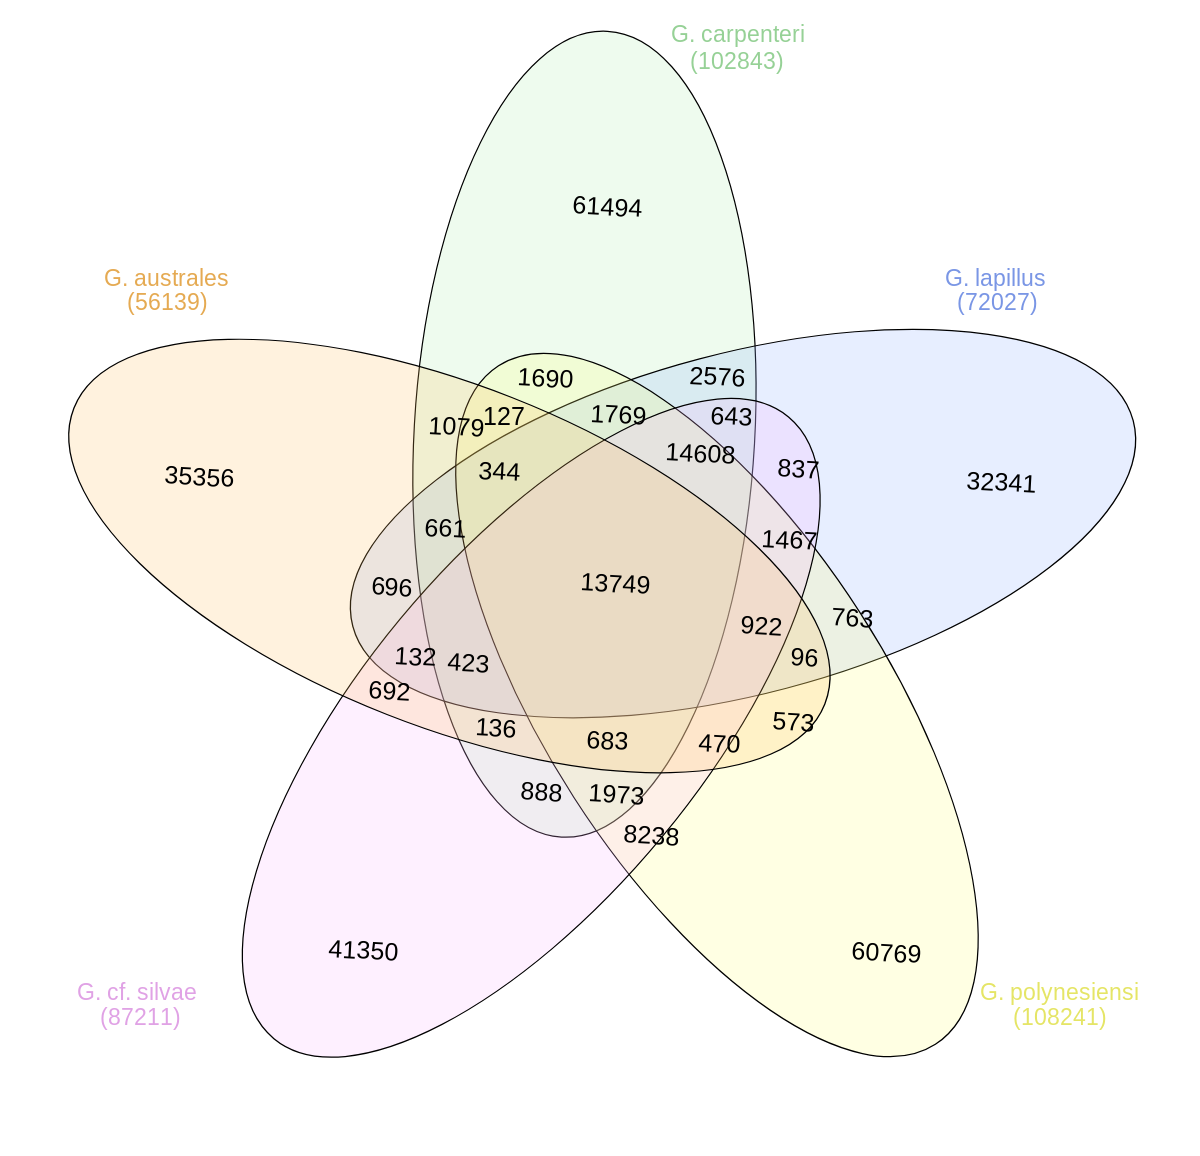
\includegraphics[scale=.4]{3Aug18_cluster-investigation/Species-venn.png} 
\caption{Venn diagram of species distribution across clusters.} 
\label{fig:SpeciesVenn}
\end{figure} 
\FloatBarrier

\begin{figure} 
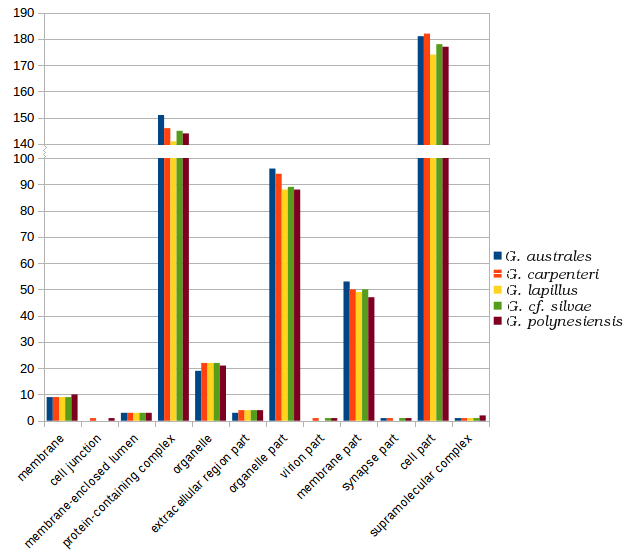
\includegraphics[scale=.9]{3Aug18_cluster-investigation/figures/gosum-species/Species-gosum1-cell-split.png} 
\caption{Summary of cellular GO annotations between \textit{Gambierdiscus} species at GOSUM level 1 from Suppl. table ~\ref{tbl:SpGO1}.} 
\label{fig:SpecGo1Cell}
\end{figure} 
\FloatBarrier

\begin{figure} 
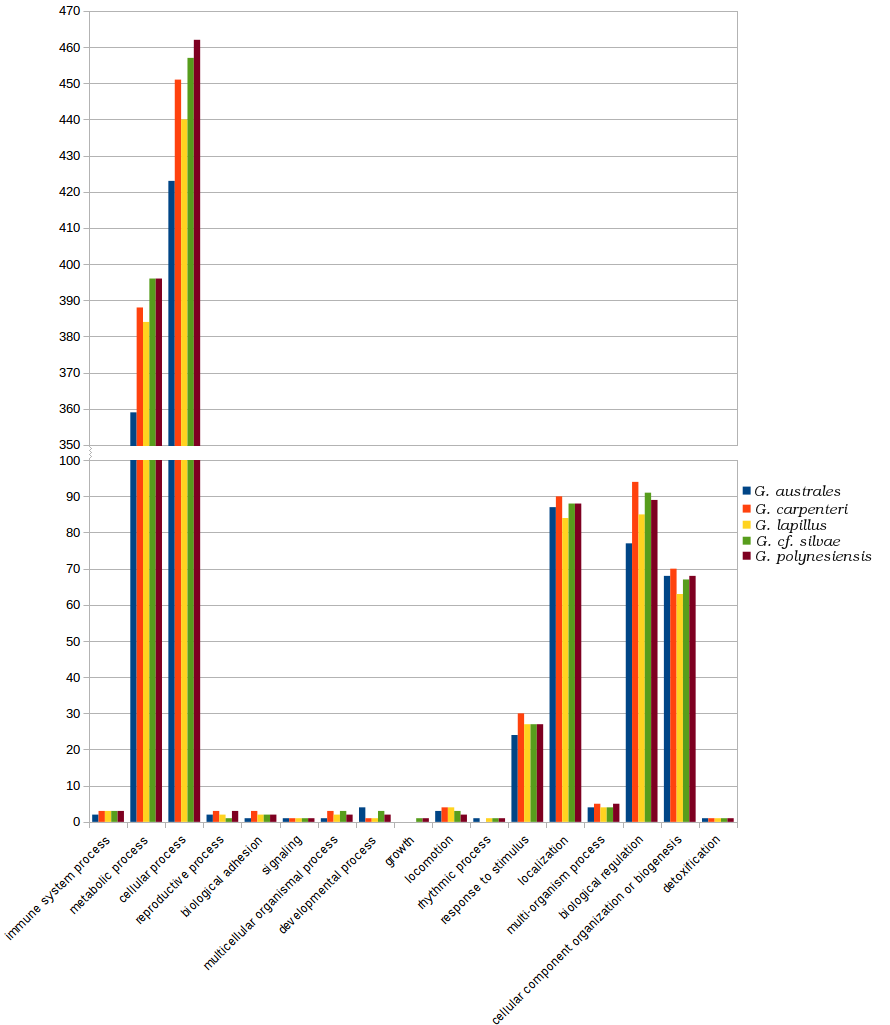
\includegraphics[scale=.7]{3Aug18_cluster-investigation/figures/gosum-species/Species-gosum1-bio-split.png} 
\caption{Summary of biological processes GO annotations between \textit{Gambierdiscus} species at GOSUM level 1 from Suppl. table ~\ref{tbl:SpGO1}.} 
\label{fig:SpecGo1Bio}
\end{figure} 
\FloatBarrier



\begin{figure} 
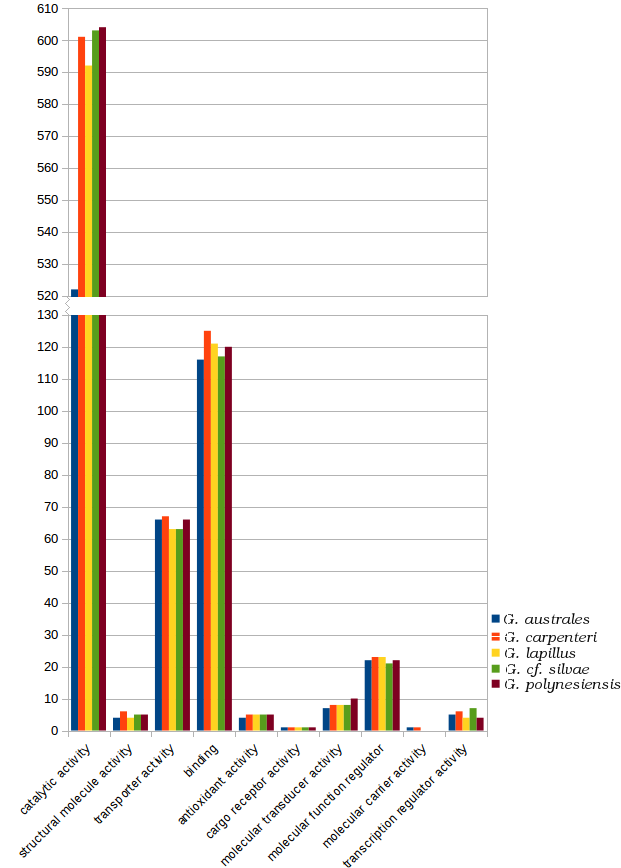
\includegraphics[scale=1]{3Aug18_cluster-investigation/figures/gosum-species/Species-gosum1-molec-split.png} 
\caption{Summary of molecular GO annotations between \textit{Gambierdiscus} species at GOSUM level 1 from Suppl. table ~\ref{tbl:SpGO1}.} 
\label{fig:SpecGo1Molec}
\end{figure} 
\FloatBarrier

\begin{figure} 
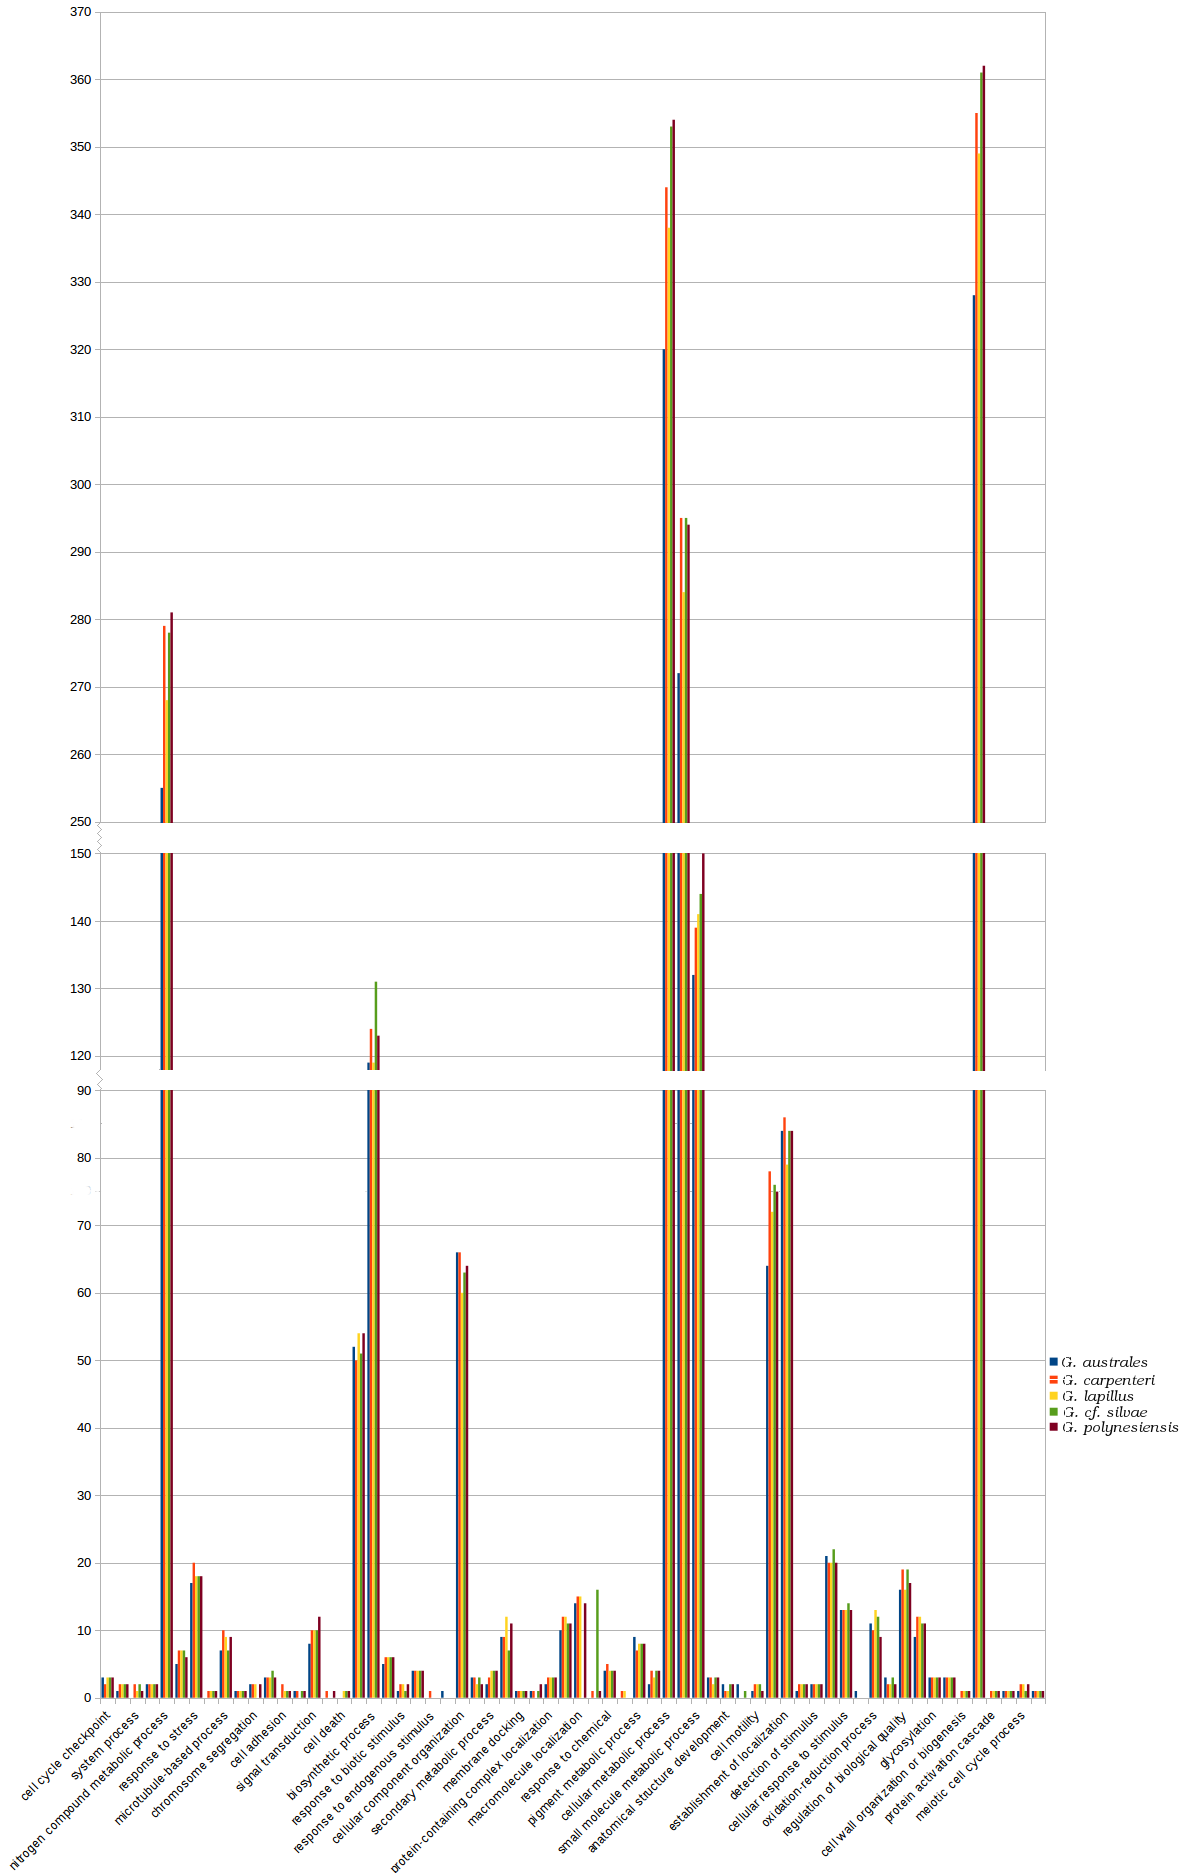
\includegraphics[scale=.45]{3Aug18_cluster-investigation/figures/gosum-species/Species-gosum2-bio2-split.png} 
\caption{Summary of biological processes GO annotations between \textit{Gambierdiscus} species at GOSUM level 2 from Suppl. table ~\ref{tbl:SpGO2}.} 
\label{fig:SpecGo2Bio}
\end{figure} 
\FloatBarrier

\begin{figure} 
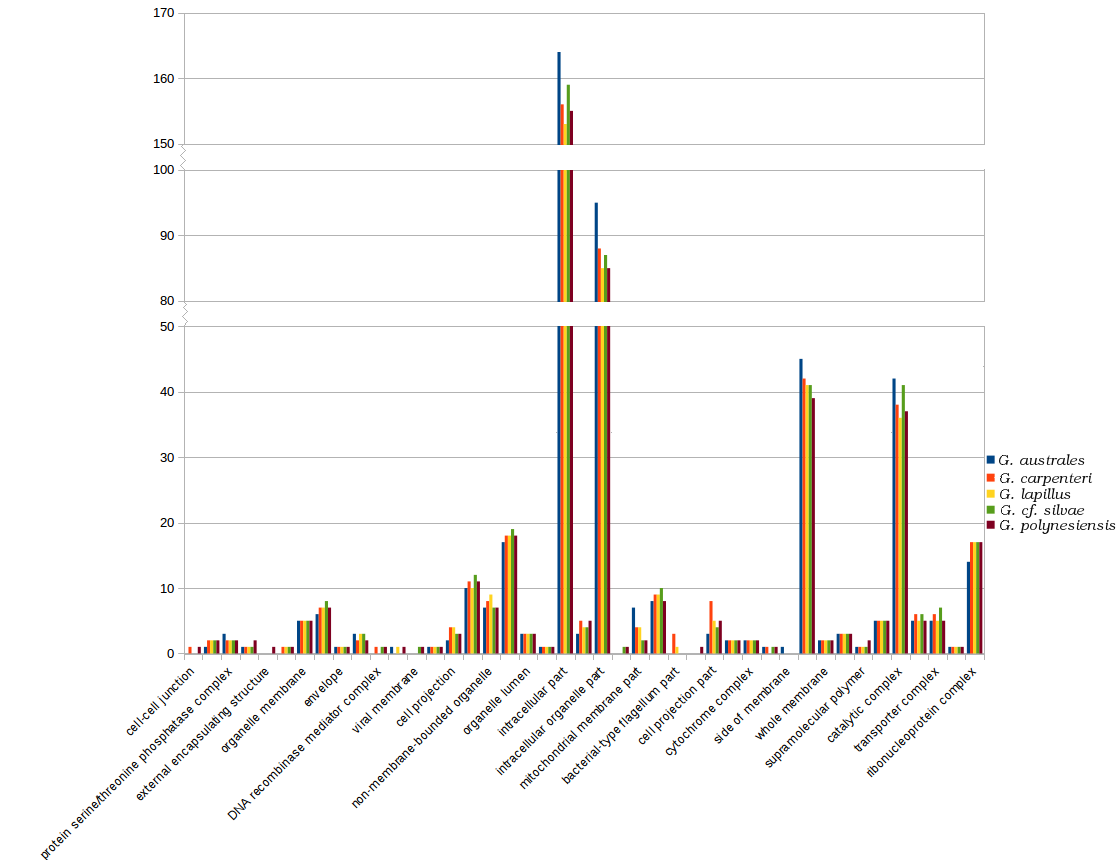
\includegraphics[scale=.6]{3Aug18_cluster-investigation/figures/gosum-species/Species-gosum2-cell2-split.png} 
\caption{Summary of cellular GO annotations between \textit{Gambierdiscus} species at GOSUM level 2 from Suppl. table ~\ref{tbl:SpGO2}.} 
\label{fig:SpecGo2Cell}
\end{figure} 
\FloatBarrier

\begin{figure} 
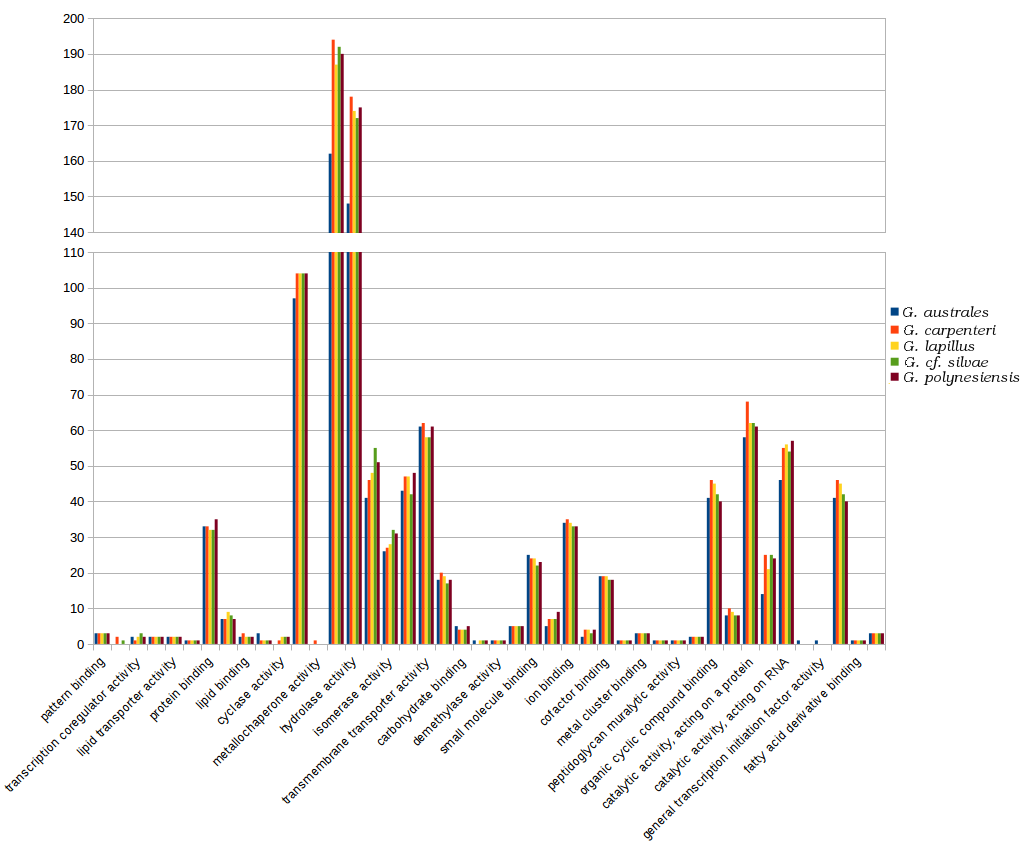
\includegraphics[scale=.6]{3Aug18_cluster-investigation/figures/gosum-species/Species-gosum2-molec-split.png} 
\caption{Summary of molecular GO annotations between \textit{Gambierdiscus} species at GOSUM level 2 from Suppl. table ~\ref{tbl:SpGO2}.}  
\label{fig:SpecGo2Molec}
\end{figure} 
\FloatBarrier

\subsection*{Transcriptome similarity clustering}
\FloatBarrier
\textbf{To do:}
\begin{itemize}
\item describe differences in graphs once I know what needs to be taken out and re-run
\item GOSUM lvl2 graphs are partially missing descriptions on x-axis. Fix when re-run
\end{itemize}
Potentially interesting points, if still there after bact and unknown outtakes:\\
- intracellular parts in pan (gosum2 cell)\\
- organelle memb in core and softcore, seem essential and not in unique (gosum2 cell)\\
- core and unique pretty evenly matched in most entries for gosum2 molec, except catalytic activity binding on DNA is  much higher in unique and a little higher for binding RNA\\
- very little difference between core and unique... possbile reasons? not annotated, should be combining core \& softcore ?

\FloatBarrier
\begin{figure} 
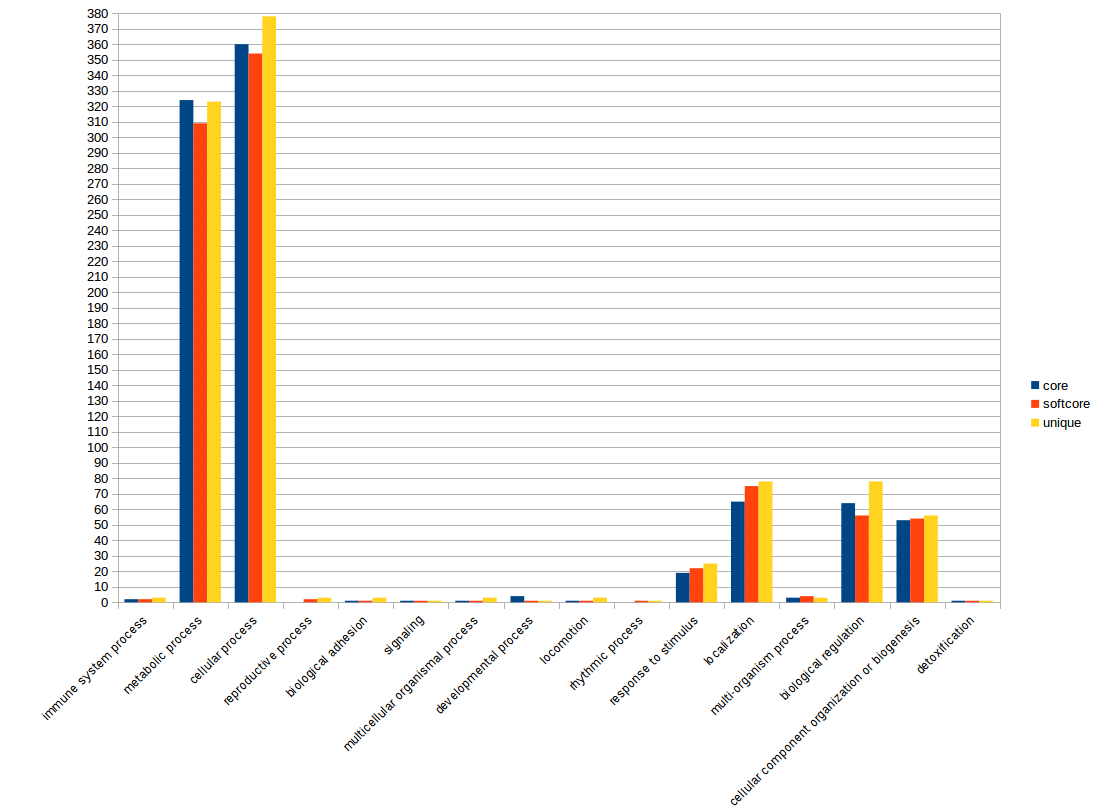
\includegraphics[scale=.58]{3Aug18_cluster-investigation/figures/gosum-pan/Pan-gosum1-bio-graph.png} 
\caption{Summary of biological processes GO annotations between core, softcore and unique clusters at GOSUM level 1.} 
\label{fig:PanGo1Bio}
\end{figure} 
\FloatBarrier

\begin{figure} 
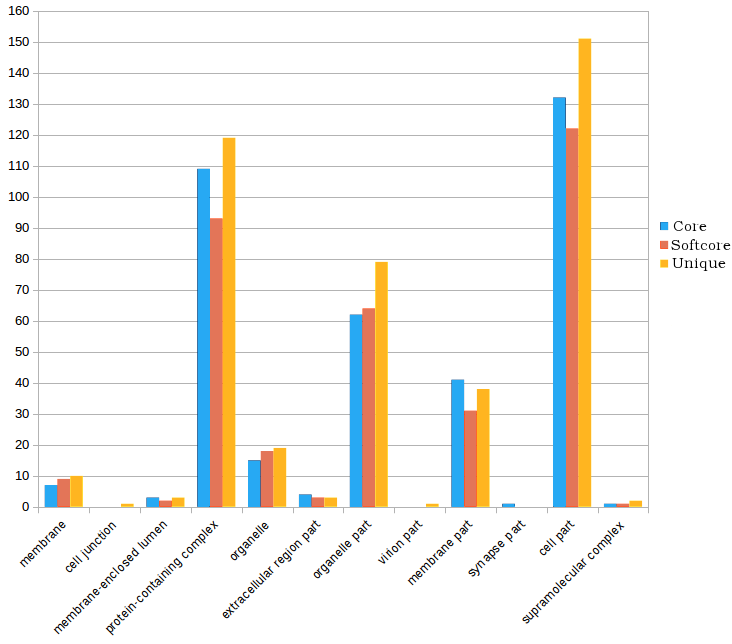
\includegraphics[scale=.8]{3Aug18_cluster-investigation/figures/gosum-pan/Pan-gosum1-cell-split.png} 
\caption{Summary of cellular GO annotations between core, softcore and unique clusters at GOSUM level 1.} 
\label{fig:PanGo1Cell}
\end{figure} 
\FloatBarrier

\begin{figure} 
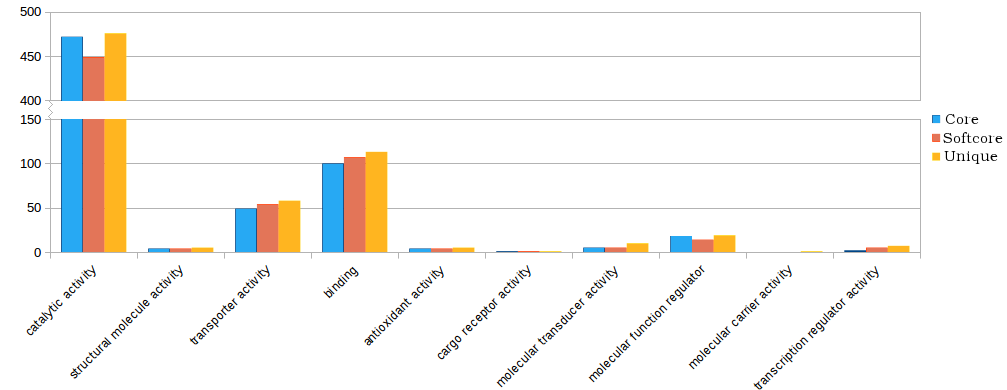
\includegraphics[scale=.6]{3Aug18_cluster-investigation/figures/gosum-pan/Pan-gosum1-molec-split.png} 
\caption{Summary of molecular GO annotations between core, softcore and unique clusters at GOSUM level 1.} 
\label{fig:PanGo1Molec}
\end{figure} 
\FloatBarrier

\begin{figure} 
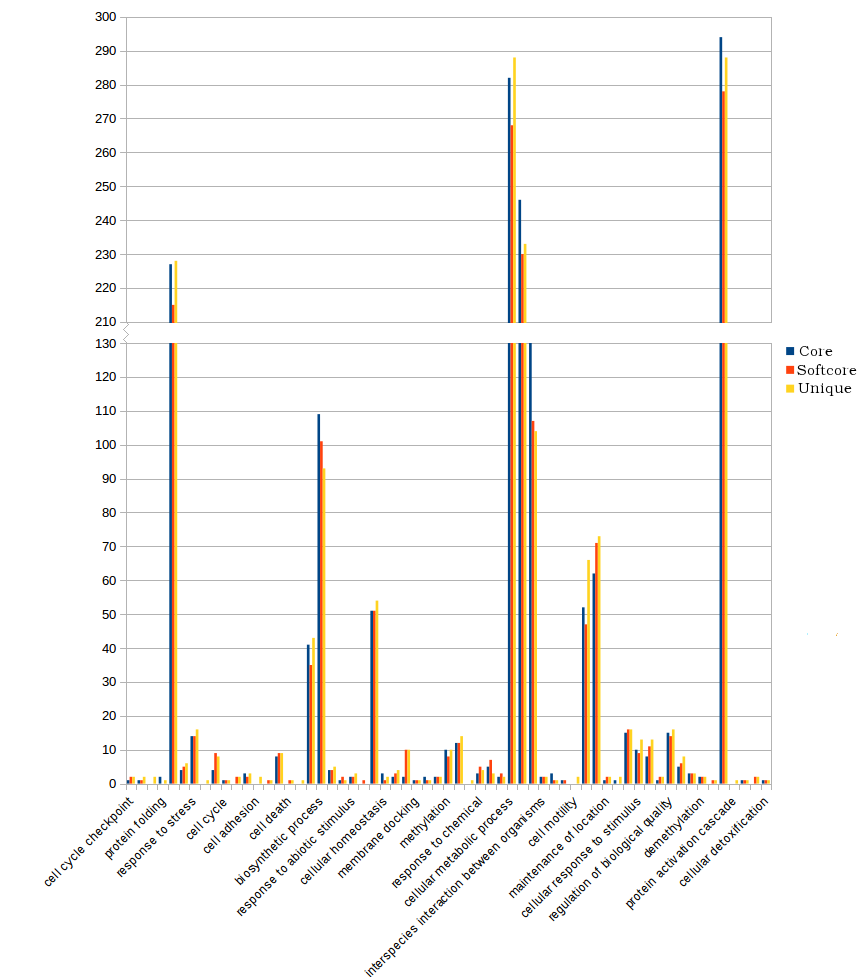
\includegraphics[scale=.75]{3Aug18_cluster-investigation/figures/gosum-pan/Pan-gosum2-bio-split.png} 
\caption{Summary of biological processes GO annotations between core, softcore and unique clusters at GOSUM level 2.} 
\label{fig:PanGo2Bio}
\end{figure} 
\FloatBarrier

\begin{figure} 
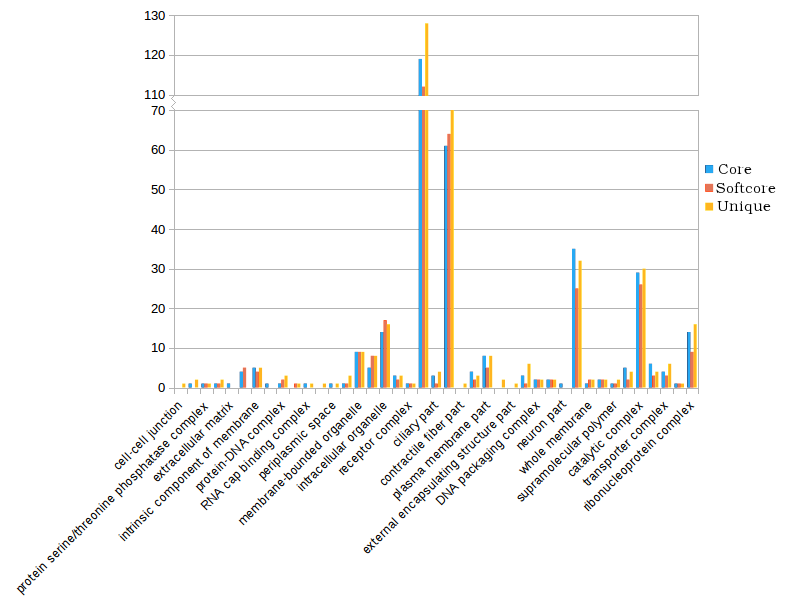
\includegraphics[scale=.8]{3Aug18_cluster-investigation/figures/gosum-pan/Pan-gosum2-cell-split.png} 
\caption{Summary of cellular GO annotations between core, softcore and unique clusters at GOSUM level 2.} 
\label{fig:PanGo2Cell}
\end{figure} 
\FloatBarrier

\begin{figure} 
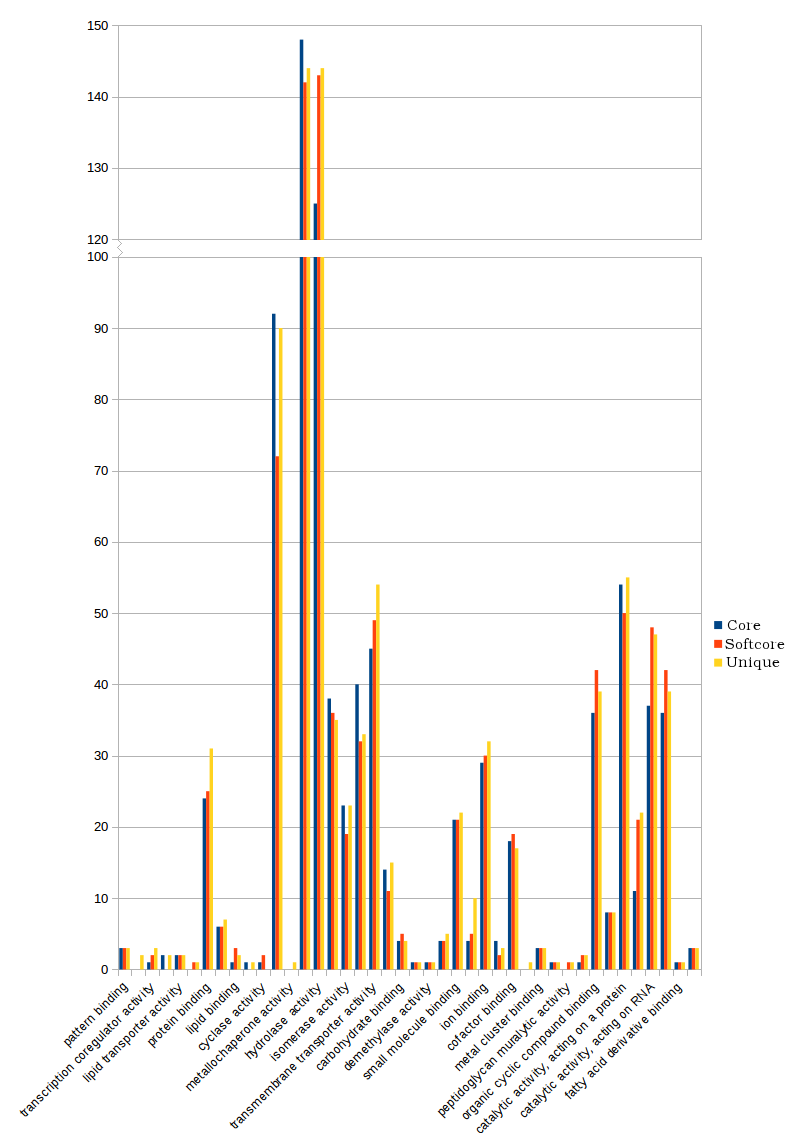
\includegraphics[scale=.78]{3Aug18_cluster-investigation/figures/gosum-pan/Pan-gosum2-molec-split.png} 
\caption{Summary of molecular GO annotations between core, softcore and unique clusters at GOSUM level 2.} 
\label{fig:PanGo2Molec}
\end{figure} 
\FloatBarrier

\subsubsection*{Core transcritome}
A set of core genes common to all five species of \textit{Gambierdiscus} were found. 
This set consisted of 13,750 amino acid clusters (Table ~\ref{tbl:ClustTable}) of which 45 \% were annotated with GO terms (Suppl. table ~\ref{tbl:PanGO1} \& ~\ref{tbl:PanGO2}). 
The highest number of contigs in any core cluster was 180 cluster of unknown function with 23, 45, 32, 31 and 49 from \textit{G. australes}, \textit{G. carpenteri} \textit{G. lapillus}, \textit{G. polynesiensis} and \textit{G.} cf. \textit{silvae} respectively. 
Twelve of the core clusters contained 100 or more contigs, of which 3 were unannotated. 
The predicted protein coding regions for the other nine clusters, in descending order of contig numbers: an enzyme with catalytic activity involved in metabolic process; a calcium binding transmembrane transport channel; a protein involved in calcium binding; a protein binding enzyme; a domain for unspecified protein binding; an enzyme with O-glucosyl hydrolase activity involved in carbohydrate metabolic process; membrane bound ion transporter with cation channel activity \& ionotropic glutamate receptor activity; a transmembrane transporter with voltage-gated calcium channel activity; and calcium ion binding transmembrane ion transporter. 
A total of 3,943 core clusters contained 10 or more contigs, so 71.32 \% of the total core clusters consisted of less than 10 contigs. 
The majority of  clusters fell within metabolic processes, cellular processes and catalytic activity with \%, \% and \% of annotated clusters respectively. \textbf{Tim} - so adding up the lvl1 gosum counts for bio, cell and molec doesn't add up to the total annotated clusters.. am I correct in thinking that this is because annotations can go to other functions too?

\subsubsection*{Softcore transcriptome}
A softcore with 4 out of the five \textit{Gambierdiscus} species examined was identified. 
The softcore consisted of an additional 16,980 clusters (Table ~\ref{tbl:ClustTable}) of which 48 \% were annotated  (Suppl. table ~\ref{tbl:PanGO1} \& ~\ref{tbl:PanGO2}). 
The most prolific cluster in the softcore contained 163 contigs with unknown function, where \textit{G. carpenteri} \textit{G. lapillus}, \textit{G. polynesiensis} and \textit{G.} cf. \textit{silvae} contained 50, 42, 41 \& 30 contigs respectively. 
A further 5 clusters contained more than 100 contigs, four of which had GO annotations. 
Of the six clusters with over 100 contigs, none had representatives contigs from \textit{G. australes}. 
\textit{G. australes} was absent from 86 \% of the softcore clusters. 
%comment about seq differences? Some fuck up common thuings
In descending order of contigs, they matched to: a protein involved in selective protein binding; a protein involved in actin binding; a protein involved in calcium binding; and a protein with cysteine-type peptidase activity. 
Of the softcore, 14,035 clusters contained 10 or more contigs. 

\subsubsection*{Pan-transcriptome}
Clusters with single species representatives, or the pan-transcriptome to the five \textit{Gambierdiscus} species examined, numbered 231,310 clusters. 
Of the unique clusters, only 15.23 \% of clusters were annotated. 
Single species clusters from \emph{G. australes}, \textit{G. carpenteri} \textit{G. lapillus}, \textit{G. polynesiensis} and \textit{G.} cf. \textit{silvae} numbered 35,356, 62,494, 32,341, 60,796 \& 41,350 clusters respectively (Table ~\ref{tbl:ClustTable}). 
%discussion: numbers mirror depth of sequencing ie. shittiest trans has least unique
The highest number of contigs in a unique cluster were 37, found in two clusters from \textit{G. carpenteri}. 
One of these was annotated for RNA and metal ion binding activity. 
Of the unique clusters, 83.1 \% contained only one contig and 97.8 \% of clusters have 5 contigs or less. 

\subsection*{Last common ancestor identification of contigs}

\FloatBarrier
\begin{table}
\caption{basta trEMBL found in each \emph{Gambierdiscus} transcriptome during processing.}
\label{tbl:bastaTable}
\begin{tabular}{ | p{3cm} | p{2cm} | p{2.5cm} | p{2.5cm} | p{2cm} | p{2cm}|}
\hline
\textbf{Species}& \textit{G. australes}& \emph{G. carpenteri}&\emph{G. lapillus}&\emph{G. polynesiensis}&\emph{G.} cf. \emph{silvae}\\
\hline
\textbf{Contigs}&102,863&263,829&148,972&270,315&191,224 \\
\hline
 \multicolumn{6}{| c |}{SwillProt}\\ %using the lax one
 \hline
 \textbf{SwissProt hits}&62,240&176,000&109,662&171,741&129,913\\ %cut -f 1 carpenteri_BASTA/blast_output/*_blast.out |uniq| wc -l
\hline
\textbf{BASTA positive ID}&19,335&60,811&40,151&57,448&43,372\\ % -m 1
\hline
\textbf{Eukaryotic origin}&10,720&35,263&22,643&32,098&24,096\\
\hline
\textbf{Bacterial origin}&826&2,784&1,799&2,438&32,098\\
\hline
\textbf{Unknown origin}&7,709&22,429&15,471&22,571&17,072\\
\hline
 \multicolumn{6}{| c |}{trEMBL}\\
 \hline
\textbf{trEMBL hits}&61,161&169,810&106,554&165,793&126,208\\  %cut -f 1 carp_BASTA_trembl/blast_output/*_trEMBL.out |uniq| wc -l
\hline
\textbf{BASTA positive ID}&37,067&106,960&71,100&103,053&106,960\\
\hline
\textbf{Eukaryotic origin}&25,015&65,986&44,320&62,274&49,516\\ %cat CAWD149_Gambierdiscus-australes_trEMBL | grep Eukaryota | wc -l
\hline
\textbf{Bacterial origin}&654&2,213&1,404&2,101&1,688\\
\hline
\textbf{Unknown origin}&11,358&38,622&25,267&38,528&27,623\\
\hline
 \multicolumn{6}{| c |}{db differences}\\
\hline
\textbf{contigs with LCA}&37,294&108,160&71,768&104,252&79,692\\
\hline
\textbf{db consensus}&13,136&37,622&25,688&36,446&28,046\\
\hline
\textbf{unknown plus LCA}&5,821&21,399&13,434&19,247&14,158\\
\hline
\textbf{LCA conflict, euk \& bact}&116&440&253&394&289\\
\hline
%\hline
%&&&&&\\
\end{tabular}
\end{table}
\FloatBarrier
\newpage

\subsubsection*{Unknown origin}
\textbf{To do:}
\begin{itemize}
\item work out if PKS domains are within unknown
\item may be bacterial origin - IF they have dinoSL, keep. If not, remove from core/pan analysis 
\end{itemize}
\subsubsection*{Bacterial origin}
\textbf{To do:}
\begin{itemize}
\item re-running with uniprot\_trembl.fasta to see how percentage identity values differ to swissprot database
\item merge trEMBL and swissprot databases and see how BASTA goes in comparison
\item check if LCA is specific enough for Proteobacteria or gamma-Proteobacteria regarding Quorum sensing taxa
\item make new directory with bacterial origin 
\item dinoSL search to see if any of bact origin are from dinos
\item look if bact contigs found in unique or core clusters
\item check if core bacteriome (how wanky is that word) or any species specific
\item check for regional link of host association. Lapillus and silvae are from Heron Island from same collection trip, poly and australes are from Rarotonga collected 9 years apart, carp is from temperate Merimbula Merimbula)
\end{itemize}

%BASTA results, default -l and -m flags ie. likely going to change as swissprot percentage match super low:\\
%- australes: 0 bact, 53 Unknown \\
%- carp: 3 bact (all unique clusters, one annotated as ATP binding), 72 Unknown \\
%UTSMER9A3_Gambierdiscus-carpenteri_DN31153_c0_g1_i1.p2	Bacteria;Proteobacteria;Gammaproteobacteria; -- in unique 236528_UTSMER9A3_Gambierdiscus-carpenteri_DN31153_c0_g1_i1.p2.faa	not annotated
%UTSMER9A3_Gambierdiscus-carpenteri_DN20628_c0_g1_i1.p1	Bacteria;Proteobacteria; -- in unique 233838_UTSMER9A3_Gambierdiscus-carpenteri_DN20628_c0_g1_i1.p1.faa	not annotated
%UTSMER9A3_Gambierdiscus-carpenteri_DN27575_c0_g1_i1.p2	Bacteria;Proteobacteria; -- in unique 235579_UTSMER9A3_Gambierdiscus-carpenteri_DN27575_c0_g1_i1.p2.faa	involved in ATP binding
%- lap: 3 bact (all in unique clusters all annotated with mRNA processing roles) 72 Unknown \\
%HG4_Gambierdiscus-lapillus_DN47596_c0_g1_i1.p1	Bacteria;Proteobacteria;Gammaproteobacteria; -- in unique 351586_HG4_Gambierdiscus-lapillus_DN47596_c0_g1_i1.p1.faa	a structural constituent of ribosome involved n mRNA translation
%HG4_Gambierdiscus-lapillus_DN13474_c0_g2_i1.p2	Bacteria;Proteobacteria; -- in unique 247208_HG4_Gambierdiscus-lapillus_DN13474_c0_g2_i1.p2.faa	binds guanosine triphosphate
%HG4_Gambierdiscus-lapillus_DN47695_c0_g1_i1.p2	Bacteria;Proteobacteria;Gammaproteobacteria; -- in unique 351653_HG4_Gambierdiscus-lapillus_DN47695_c0_g1_i1.p2.faa	involved in mRNA translation
%- pol: 0 bact, 95 Unknown \\
%- sil: 0 bact, 56 Unknown \\
%- -m 1 \& -l 80 for carp with swissprot db had much higher bact contamn: 2,784 seqs bact, 22,429 seqs unknown, 35,263 seqs eukar .. contamination potentially a problem here \\

%\subsection*{\emph{Gambierdiscus polynesiensis} intra-species core \& pan transcriptome}
\subsection*{Looking into toxin producers}
not sure how valid an approach this following section is
\subsubsection*{Clusters that don't have \textit{G. carpenteri} in}
Rationale: This strain of carpenteri is the only one of the 5 which is a verified non-CTX producer, by LC-MS and bioassay.\\
To do:
\begin{itemize}
\item find clusters excluding carp
\item look for clusters with higher number of contigs from poly and silvae as those are the two more toxic ones
\item check for dinoSL and LCA of clusters
\end{itemize}

\subsubsection*{\textit{G. polynesiensis} solo clusters}
\begin{itemize}
\item number of clusters
\item percentage annotated
\item pathways present (another GOSUM adventure?)
\item as \textit{G. silvae} and to a much reduced extend, \textit{G. lapillus}, also produce CTX, is the solo polynesiensis section relevant?
\end{itemize}


\subsubsection*{Polyketide synthase active domain search}

\begin{table}
\caption{PKS active domains found in the \emph{Gambierdiscus} species queries.}
\label{tbl:PKSTable}
\begin{tabular}{ | p{1.65cm} | p{1.5cm} | p{1.5cm} | p{1.5cm} | p{1.7cm} | p{1.5cm}| p{1.5cm}| p{1.5cm}|}
\hline
\textbf{Active domain}& \textit{G. australes}& \emph{G. carpenteri}&\emph{G. lapillus}&\emph{G. polynesiensis}&\emph{G.} cf. \emph{silvae}&\textbf{Total contigs}&\textbf{\# clusters}\\
\hline
ACP&&&&&&&\\
\hline
AT&&&&&&&\\
\hline
DR&&&&&&&\\
\hline
ET&&&&&&&\\
\hline
KS&130&195&150&221&154&850&314\\
\hline
KR&&&&&&&\\
\hline
TE&&&&&&&\\
\hline
\end{tabular}
\end{table}
\FloatBarrier

\paragraph*{KS domains.}
\FloatBarrier
A total of 850 contigs were identified with KS domains which assembled into 314 clusters (table ~\ref{tbl:PKSTable}). 
Nine clusters contained more than 10 contigs, with the highest number of 130 contigs from all species.
9 clusters contained 10 contigs or more, of which only two did not contain all the taxa examined.
57 of the 314 clusters contained contigs from multiple species, so 81.8 \% of KS clusters were species specific while 78.7 \% contained only a single contig (Fig. ~\ref{fig:KSVenn}). 
The non-ciguatoxic \textit{G. carpenteri} was absent from 73.6 \% of the clusters. 
Of the clusters without \textit{G. carpenteri}, none contained all four other species. 
However one cluster contained \textit{G. lapillus}, \textit{G. polynesiensis} and \emph{G.} cf. \emph{silvae} with equally represented transcript numbers. 
Four contigs contained \textit{G. polynesiensis} and \emph{G.} cf. \emph{silvae} only, one of which had a higher contig representation of \textit{G. polynesiensis} than \emph{G.} cf. \emph{silvae}. 
\textit{G. polynesiensis} was the only representative species in 71 clusters, of which three clusters contained 2 contigs and one cluster contained 3 contigs. 
\emph{G.} cf. \emph{silvae} was representative as the only species in 23 clusters, one of which contained 3 contigs while the other clusters contained single contigs.
\textit{G. australes}, \textit{G. carpenteri} and \textit{G. lapillus} were the solo representatives of 81, 39 \& 35 KS clusters respectively. \\
\begin{figure} 
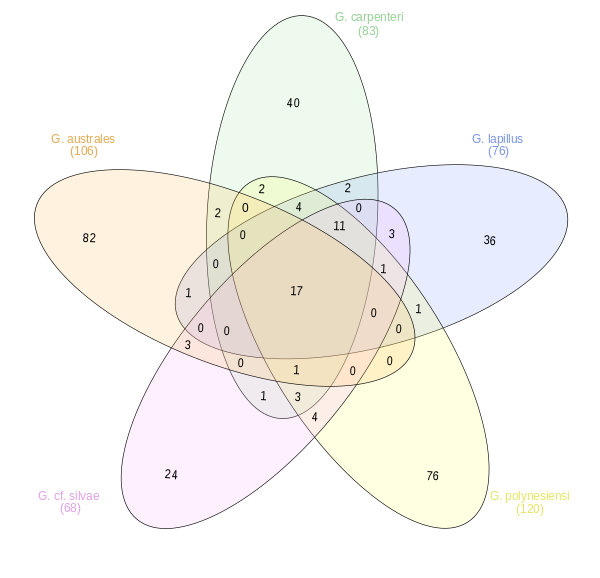
\includegraphics[scale=1]{3Aug18_cluster-investigation/pks/KS-venn.png} 
\caption{Venn diagram of species in KS clusters.} 
\label{fig:KSVenn}
\end{figure} 
\FloatBarrier

\textbf{To do:}
\begin{itemize}
\item are there any multi-domain  transcripts?
\end{itemize}

\section*{Discussion}
To go here:
\begin{itemize}
\item overall summary of study
\item core and pan more likely to be accurate without being axenic unless same contamination \textbf{vs} removing bact LCA
\item spliced leader sites really low. potentially interesting - the two highest ones are from same phylogenetic clade, while the other three are representatives from the other two main clades. Also poly and silvae are from separate seq runs, so not an artefact from that front.
\item \textit{G. australes} seq is quite bad in comparison as can be seen in the GOSUM figs and the comparative number of contigs, predicted proteins and softcore clusters
\item \textbf{Tim} not sure if I can do something like Fig 2 - only 5 isolates to put in, and I think I need to look at that again with more sleep to work out what's going on and if I could transfer the concept., there are over 200,000 pan-tran clusters, I don't think I can work out whether they are genophyletic or monophyletic for that many
\end{itemize}

\subsection*{core \textit{Gambierdiscus} transcriptome}
 \cite{lidie2005gene} comprehensive index of genes in \textit{K. brevis} to compare to as well as functional summaries 

\subsubsection*{discuss common \& different functions found}
\textbf{Koid 14} pan-transcriptome of 4 prymnesiophyte algae. 
Compare functional findings (KOG vs. this) and contigs as well as predicted protein coding regions are just a fraction of the ones here. 
eg.30,000-56,000 contigs vs. lowest for in this study is 148,972. 
Other study transcriptomes are part of MMETSP, but even australes here is over 100,000 contigs which is from the same study so more likely it's a Gambi thing rather than a seq thing.
same with australes and Koid for peptides predicted, almost double. 
Way higher for other gambis.\\


\subsubsection*{Expression of genes involved in polyketide production}
\begin{itemize}
\item discuss if different gene sets were expressed between toxic and non- toxic strains (ie. not carp)
\item discuss KS containing contigs per species plus distribution and number of contigs in KS clusters
\item point at Venn diagram intersections that could be of interest for further investigation for both MTX and CTX
\item discuss KS conserved region phylogeny
\item \textbf{Tim} I'm not sure we know enough about these pathways to do something like fig 5 
\end{itemize}

\subsubsection*{Bacterial association with host}
\begin{itemize}
\item really depends what the basta results are and if anything interesting is found
\end{itemize}

\subsubsection*{discuss usefulness for future studies}
\begin{itemize}
\item Usefullness of core transcriptome for RNA sequencing studies
\item Investigate poly only KS clusters or clusters with high number of poly reps
\end{itemize}

\subsubsection*{discuss potential short comings} 
\begin{itemize}
\item from different seq runs and methods and seq depth may vary, especially \textit{G. australes}
\item intra-speces variation so one isolate per species may not be representative
\item unknown if processes other than PKS play a role in toxin production
\end{itemize}
%\subsection*{core \textit{G. polynesiensis} transcriptome}
%- discuss common gene pathways found \\
%-discuss usefulness for future studies\\
%-discuss potential short commings

%\newpage
\section*{Conclusion}


\section*{Supplementary}
- need to add australes

\FloatBarrier
\begin{longtable}{ | p{2.2cm} | p{4cm} |p{2cm} | p{2cm} | p{2cm} | p{2cm} |}
\caption{GO terms and number of contigs per species at GO ontology level 1.}\\
\hline
\label{tbl:SpGO1}
GO acession&GO terms&\emph{G. carpenteri}&\emph{G. lapillus}&\emph{G. polynesiensis}&\emph{G.} cf. \emph{silvae}\\
\hline
 \multicolumn{6}{| c |}{Biological processes}\\
 \hline
GO:0002376&immune system process&3&3&3&3\\
 \hline
GO:0008152&metabolic process&388&384&396&396\\
 \hline
GO:0009987&cellular process&451&440&457&462\\
 \hline
GO:0022414&reproductive process&3&2&1&3\\
 \hline
GO:0022610&biological adhesion&3&2&2&2\\
 \hline
GO:0023052&signaling&1&1&1&1\\
 \hline
GO:0032501&multicellular organismal process&3&2&3&2\\
 \hline
GO:0032502&developmental process&1&1&3&2\\
 \hline
GO:0040007&growth&0&0&1&1\\
 \hline
GO:0040011&locomotion&4&4&3&2\\
 \hline
GO:0048511&rhythmic process&0&1&1&1\\
 \hline
GO:0050896&response to stimulus&30&27&27&27\\
 \hline
GO:0051179&localization&90&84&88&88\\
 \hline
GO:0051704&multi-organism process&5&4&4&5\\
 \hline
GO:0065007&biological regulation&94&85&91&89\\
 \hline
GO:0071840&cellular component organization/biogenesis&70&63&67&68\\
 \hline
GO:0098754&detoxification&1&1&1&1\\
\hline
 \multicolumn{6}{| c |}{Cellular components}\\
 \hline
GO:0016020&membrane&9&9&9&10\\
 \hline
GO:0030054&cell junction&1&0&0&1\\
 \hline
GO:0031974&membrane-enclosed lumen&3&3&3&3\\
 \hline
GO:0032991&protein-containing complex&146&141&145&144\\
 \hline
GO:0043226&organelle&22&22&22&21\\
 \hline
GO:0044421&extracellular region part&4&4&4&4\\
 \hline
GO:0044422&organelle part&94&88&89&88\\
 \hline
GO:0044423&virion part&1&0&1&1\\
 \hline
GO:0044425&membrane part&50&49&50&47\\
 \hline
GO:0044456&synapse part&1&0&1&1\\
 \hline
GO:0044464&cell part&182&174&178&177\\
 \hline
GO:0099080&supramolecular complex&1&1&1&2\\
\hline
 \multicolumn{6}{| c |}{Molecular function}\\
\hline
GO:0003824&catalytic activity&601&592&603&604\\
\hline
GO:0005198&structural molecule activity&6&4&5&5\\
\hline
GO:0005215&transporter activity&67&63&63&66\\
\hline
GO:0005488&binding&125&121&117&120\\
\hline
GO:0016209&antioxidant activity&5&5&5&5\\
\hline
GO:0038024&cargo receptor activity&1&1&1&1\\
\hline
GO:0060089&molecular transducer activity&8&8&8&10\\
\hline
%988_MMETSP0766_Gambierdiscus-australes_DN11896_c0_g2_i1.p1.faa	6	40	29	24	31	130 \\ WTF IS THIS
%8866_MMETSP0766_Gambierdiscus-australes_DN22301_c0_g2_i1.p1.faa	3	24	14	24	16	81
%3681_MMETSP0766_Gambierdiscus-australes_DN15885_c0_g1_i1.p1.faa	7	14	16	9	12	58
%1921_MMETSP0766_Gambierdiscus-australes_DN13038_c0_g1_i1.p1.faa	3	10	6	4	6	29
%46550_MMETSP0766_Gambierdiscus-australes_DN42196_c9_g13_i1.p1.faa	3	4	1	8	5	21
%215601_UTSMER9A3_Gambierdiscus-carpenteri_DN18221_c2_g10_i1.p1.faa	0	4	1	8	5	18
%360_MMETSP0766_Gambierdiscus-australes_DN10555_c0_g1_i1.p1.faa	1	4	3	3	4	15
%15645_MMETSP0766_Gambierdiscus-australes_DN27800_c0_g2_i1.p1.faa	4	2	0	4	1	11
%132980_UTSMER9A3_Gambierdiscus-carpenteri_DN14854_c1_g5_i1.p1.faa	0	1	4	3	2	10
GO:0098772&molecular function regulator&23&23&21&22\\
\hline
GO:0140104&molecular carrier activity&1&0&0&0\\
\hline
GO:0140110&transcription regulator activity&6&4&7&4\\
\hline
\end{longtable}

\FloatBarrier
\begin{longtable}{ | p{2.2cm} | p{4cm} |p{2cm} | p{2cm} | p{2cm} | p{2cm} |}
\caption{GO terms and number of contigs per species at GO ontology level 2, child terms of Table ~\ref{tbl:SpGO1}.}\\
\hline
\label{tbl:SpGO2}
GO acession&GO terms&\emph{G. carpenteri}&\emph{G. lapillus}&\emph{G. polynesiensis}&\emph{G.} cf. \emph{silvae}\\
\hline
 \multicolumn{6}{| c |}{Biological processes}\\
 \hline
GO:0000075&cell cycle checkpoint&2&3&3&3\\
 \hline
GO:0002252&immune effector process&2&2&2&2\\
 \hline
GO:0003008&system process&2&1&2&1\\
 \hline
GO:0006457&protein folding&2&2&2&2\\
 \hline
GO:0006807&nitrogen compound metabolic process&279&268&278&281\\
 \hline
GO:0006928&movement of cell or subcellular component&7&7&7&6\\
 \hline
GO:0006950&response to stress&20&18&18&18\\
 \hline
GO:0006955&immune response&1&1&1&1\\
 \hline
GO:0007017&microtubule-based process&10&9&7&9\\
 \hline
GO:0007049&cell cycle&1&1&1&1\\
 \hline
GO:0007059&chromosome segregation&2&2&0&2\\
 \hline
GO:0007154&cell communication&3&3&4&3\\
 \hline
GO:0007155&cell adhesion&2&1&1&1\\
 \hline
GO:0007163&establishment or maintenance of cell polarity&1&0&1&1\\
 \hline
GO:0007165&signal transduction&10&10&10&12\\
 \hline
GO:0008037&cell recognition&1&0&0&1\\
 \hline
GO:0008219&cell death&0&1&1&1\\
 \hline
GO:0009056&catabolic process&50&54&51&54\\
 \hline
GO:0009058&biosynthetic process&124&119&131&123\\
 \hline
GO:0009605&response to external stimulus&6&6&6&6\\
 \hline
GO:0009607&response to biotic stimulus&2&2&1&2\\
 \hline
GO:0009628&response to abiotic stimulus&4&4&4&4\\
 \hline
GO:0009719&response to endogenous stimulus&1&0&0&0\\
 \hline
GO:0016043&cellular component organization&66&60&63&64\\
 \hline
GO:0019725&cellular homeostasis&3&2&3&2\\
 \hline
GO:0019748&secondary metabolic process&3&4&4&4\\
 \hline
GO:0022402&cell cycle process&9&12&7&11\\
 \hline
GO:0022406&membrane docking&1&1&1&1\\
 \hline
GO:0030029&actin filament-based process&1&0&1&2\\
 \hline
GO:0031503&protein-containing complex localization&3&3&3&3\\
 \hline
GO:0032259&methylation&12&12&11&11\\
 \hline
GO:0033036&macromolecule localization&15&15&0&14\\
 \hline
GO:0035036&sperm-egg recognition&1&0&16&1\\
 \hline
GO:0042221&response to chemical&5&4&4&4\\
 \hline
GO:0042330&taxis&1&1&0&0\\
 \hline
GO:0042440&pigment metabolic process&7&8&8&8\\
 \hline
GO:0044085&cellular component biogenesis&4&3&4&4\\
 \hline
GO:0044237&cellular metabolic process&344&338&353&354\\
 \hline
GO:0044238&primary metabolic process&295&284&295&294\\
 \hline
GO:0044281&small molecule metabolic process&139&141&144&150\\
 \hline
GO:0044419&interspecies interaction between organisms&3&2&3&3\\
 \hline
GO:0048856&anatomical structure development&1&1&2&2\\
 \hline
GO:0048869&cellular developmental process&0&0&1&\\
 \hline
GO:0048870&cell motility&2&2&2&1\\
 \hline
GO:0050789&regulation of biological process&78&72&76&75\\
 \hline
GO:0051234&establishment of localization&86&79&84&84\\
 \hline
GO:0051235&maintenance of location&2&2&2&2\\
 \hline
GO:0051606&detection of stimulus&2&2&2&2\\
 \hline
GO:0051641&cellular localization&20&20&22&20\\
 \hline
GO:0051716&cellular response to stimulus&13&13&14&13\\
 \hline
GO:0055114&oxidation-reduction process&10&13&12&9\\
 \hline
GO:0061919&process utilizing autophagic mechanism&2&2&3&2\\
 \hline
GO:0065008&regulation of biological quality&19&16&19&17\\
 \hline
GO:0065009&regulation of molecular function&12&12&11&11\\
 \hline
GO:0070085&glycosylation&3&3&3&3\\
 \hline
GO:0070988&demethylation&3&3&3&3\\

GO:0071554&cell wall organization or biogenesis&1&1&1&1\\

GO:0071704&organic substance metabolic process&355&349&361&362\\
 \hline
GO:0072376&protein activation cascade&1&1&1&1\\
 \hline
GO:0140029&exocytic process&1&1&1&1\\
 \hline
GO:1903046&meiotic cell cycle process&2&2&1&2\\
 \hline
GO:1990748&cellular detoxification&1&1&1&1\\
\hline
 \multicolumn{6}{| c |}{Cellular components}\\
 \hline
GO:0005911&cell-cell junction&1&0&0&1\\
 \hline
GO:0005929&cilium&2&2&2&2\\
 \hline
GO:0008287&protein serine/threonine phosphatase complex&2&2&2&2\\
 \hline
GO:0019867&outer membrane&1&1&1&2\\
 \hline
GO:0030312&external encapsulating structure&0&0&0&1\\
 \hline
GO:0031012&extracellular matrix&1&1&1&1\\
 \hline
GO:0031090&organelle membrane&5&5&5&5\\
 \hline
GO:0031224&intrinsic component of membrane&7&7&8&7\\
 \hline
GO:0031975&envelope&1&1&1&1\\
 \hline
GO:0032993&protein-DNA complex&2&3&3&2\\
 \hline
GO:0033061&DNA recombinase mediator complex&1&0&1&1\\
 \hline
GO:0034518&RNA cap binding complex&0&1&0&1\\
 \hline
GO:0036338&viral membrane&0&0&1&1\\
 \hline
GO:0042597&periplasmic space&1&1&1&1\\
 \hline
GO:0042995&cell projection&4&4&3&3\\
 \hline
GO:0043227&membrane-bounded organelle&11&10&12&11\\
 \hline
GO:0043228&non-membrane-bounded organelle&8&9&7&7\\
 \hline
GO:0043229&intracellular organelle&18&18&19&18\\
 \hline
GO:0043233&organelle lumen&3&3&3&3\\
 \hline
GO:0043235&receptor complex&1&1&1&1\\
 \hline
GO:0044424&intracellular part&156&153&159&155\\
 \hline
GO:0044441&ciliary part&5&4&4&5\\
 \hline
GO:0044446&intracellular organelle part&88&85&87&85\\
 \hline
GO:0044449&contractile fiber part&0&0&1&1\\
 \hline
GO:0044455&mitochondrial membrane part&4&4&2&2\\
 \hline
GO:0044459&plasma membrane part&9&9&10&8\\
 \hline
GO:0044461&bacterial-type flagellum part&3&1&0&0\\
 \hline
GO:0044462&external encapsulating structure part&0&0&0&1\\
 \hline
GO:0044463&cell projection part&8&5&4&5\\
 \hline
GO:0044815&DNA packaging complex&2&2&2&2\\
 \hline
GO:0070069&cytochrome complex&2&2&2&2\\
 \hline
GO:0097458&neuron part&1&0&1&1\\
 \hline
GO:0098796&membrane protein complex&42&41&41&39\\
 \hline
GO:0098805&whole membrane&2&2&2&2\\
 \hline
GO:0099023&tethering complex&3&3&3&3\\
 \hline
GO:0099081&supramolecular polymer&1&1&1&2\\
 \hline
GO:0120114&Sm-like protein family complex&5&5&5&5\\
 \hline
GO:1902494&catalytic complex&38&36&41&37\\
 \hline
GO:1990204&oxidoreductase complex&6&5&6&5\\
 \hline
GO:1990351&transporter complex&6&5&7&5\\
 \hline
GO:1990391&DNA repair complex&1&1&1&1\\
 \hline
GO:1990904&ribonucleoprotein complex&17&17&17&17\\
\hline
 \multicolumn{6}{| c |}{Molecular function}\\
\hline
GO:0001871&pattern binding&3&3&3&3\\
\hline
GO:0003700&DNA-binding transcription factor activity&2&0&1&0\\
\hline
GO:0003712&transcription coregulator activity&1&2&3&2\\
\hline
GO:0004133&glycogen debranching enzyme activity&2&2&2&2\\
\hline
GO:0005319&lipid transporter activity&2&2&2&2\\
\hline
GO:0005326&neurotransmitter transporter activity&1&1&1&1\\
\hline
GO:0005515&protein binding&33&32&32&35\\
\hline
GO:0008144&drug binding&7&9&8&7\\
\hline
GO:0008289&lipid binding&3&2&2&2\\
\hline
GO:0008565&protein transporter activity&1&1&1&1\\
\hline
GO:0009975&cyclase activity&1&2&2&2\\
\hline
GO:0016491&oxidoreductase activity&104&104&104&104\\
\hline
GO:0016530&metallochaperone activity&1&0&0&0\\
\hline
GO:0016740&transferase activity&194&187&192&190\\
\hline
GO:0016787&hydrolase activity&178&174&172&175\\
\hline
GO:0016829&lyase activity&46&48&55&51\\
\hline
GO:0016853&isomerase activity&27&28&32&31\\
\hline
GO:0016874&ligase activity&47&47&42&48\\
\hline
GO:0022857&transmembrane transporter activity&62&58&58&61\\
\hline
GO:0030234&enzyme regulator activity&20&19&17&18\\
\hline
GO:0030246&carbohydrate binding&4&4&4&5\\
\hline
GO:0030545&receptor regulator activity&0&1&1&1\\
\hline
GO:0032451&demethylase activity&1&1&1&1\\
\hline
GO:0033218&amide binding&5&5&5&5\\
\hline
GO:0036094&small molecule binding&24&24&22&23\\
\hline
GO:0038023&signaling receptor activity&7&7&7&9\\
\hline
GO:0043167&ion binding&35&34&33&33\\
\hline
GO:0044877&protein-containing complex binding&4&4&3&4\\
\hline
GO:0048037&cofactor binding&19&19&18&18\\
\hline
GO:0050824&water binding&1&1&1&1\\
\hline
GO:0051540&metal cluster binding&3&3&3&3\\
\hline
GO:0060090&molecular adaptor activity&1&1&1&1\\
\hline
GO:0061783&peptidoglycan muralytic activity&1&1&1&1\\
\hline
GO:0072341&modified amino acid binding&2&2&2&2\\
\hline
GO:0097159&organic cyclic compound binding&46&45&42&40\\
\hline
GO:0097367&carbohydrate derivative binding&10&9&8&8\\
\hline
GO:0140096&catalytic activity, acting on a protein&68&62&62&61\\
\hline
GO:0140097&catalytic activity, acting on DNA&25&21&25&24\\
\hline
GO:0140098&catalytic activity, acting on RNA&55&56&54&57\\
\hline
GO:1901363&heterocyclic compound binding&46&45&42&40\\
\hline
GO:1901567&fatty acid derivative binding&1&1&1&1\\
\hline
GO:1901681&sulfur compound binding&3&3&3&3\\
\hline
\end{longtable}


\FloatBarrier
\begin{longtable}{ | p{2.2cm} | p{4cm} |p{2cm} | p{2cm} | p{2cm} | }
\caption{GO terms and number of contigs found in core, softcore and pan-transcriptome of \textit{Gambierdiscus} at GO ontology level 1.}\\
\hline
\label{tbl:PanGO1}
GO acession&GO terms&Core&Softcore&Pan\\
\hline
 \multicolumn{5}{| c |}{Biological processes}\\
 \hline
GO:0002376&immune system process&2&2&3\\
 \hline
GO:0008152&metabolic process&324&309&323\\
 \hline
GO:0009987&cellular process&360&354&378\\
 \hline
GO:0022414&reproductive process&0&2&3\\
 \hline
GO:0022610&biological adhesion&1&1&3\\
 \hline
GO:0023052&signaling&1&1&1\\
 \hline
GO:0032501&multicellular organismal process&1&1&3\\
 \hline
GO:0032502&developmental process&4&1&1\\
 \hline
GO:0040011&locomotion&1&1&3\\
 \hline
GO:0048511&rhythmic process&0&1&1\\
 \hline
GO:0050896&response to stimulus&19&22&25\\
 \hline
GO:0051179&localization&65&75&78\\
 \hline
GO:0051704&multi-organism process&3&4&3\\
 \hline
GO:0065007&biological regulation&64&56&78\\
 \hline
GO:0071840&cellular component organization or biogenesis&53&54&56\\
 \hline
GO:0098754&detoxification&1&1&1\\
\hline
 \multicolumn{5}{| c |}{Cellular components}\\
 \hline
GO:0016020&membrane&7&9&10\\ 
 \hline 
GO:0030054&cell junction&0&0&1\\ 
 \hline 
GO:0031974&membrane-enclosed lumen&3&2&3\\ 
 \hline 
GO:0032991&protein-containing complex&109&93&119\\ 
 \hline 
GO:0043226&organelle&15&18&19\\ 
 \hline 
GO:0044421&extracellular region part&4&3&3\\ 
 \hline 
GO:0044422&organelle part&62&64&79\\ 
 \hline 
GO:0044423&virion part&0&0&1\\ 
 \hline 
GO:0044425&membrane part&41&31&38\\ 
 \hline 
GO:0044456&synapse part&1&0&0\\ 
 \hline 
GO:0044464&cell part&132&122&151\\ 
 \hline 
GO:0099080&supramolecular complex&1&1&2\\ 
\hline
 \multicolumn{5}{| c |}{Molecular function}\\
\hline
GO:0003824&catalytic activity&472&449&476\\ 
 \hline 
GO:0005198&structural molecule activity&4&4&5\\ 
 \hline 
GO:0005215&transporter activity&49&54&58\\ 
 \hline 
GO:0005488&binding&100&107&113\\ 
 \hline 
GO:0016209&antioxidant activity&4&4&5\\ 
 \hline 
GO:0038024&cargo receptor activity&1&1&1\\ 
 \hline 
GO:0060089&molecular transducer activity&5&5&10\\ 
 \hline 
GO:0098772&molecular function regulator&18&14&19\\ 
 \hline 
GO:0140104&molecular carrier activity&0&0&1\\ 
 \hline 
GO:0140110&transcription regulator activity&2&5&7\\ 
\hline
\end{longtable}

\FloatBarrier
\begin{longtable}{ | p{2.2cm} | p{4cm} |p{2cm} | p{2cm} | p{2cm} | }
\caption{GO terms and number of contigs found in core, softcore and pan-transcriptome of \textit{Gambierdiscus} at GO ontology level 2, childer to Table ~\ref{tbl:PanGO1}.}\\
\hline
\label{tbl:PanGO2}
GO acession&GO terms&Core&Softcore&Pan\\
\hline
 \multicolumn{5}{| c |}{Biological processes}\\
 \hline
GO:0000075&cell cycle checkpoint&1&2&2\\ 
 \hline 
GO:0002252&immune effector process&1&1&2\\ 
 \hline 
GO:0003008&system process&0&0&2\\ 
 \hline 
GO:0006457&protein folding&2&0&1\\ 
 \hline 
GO:0006807&nitrogen compound metabolic process&227&215&228\\ 
 \hline 
GO:0006928&movement of cell or subcellular component&4&5&6\\ 
 \hline 
GO:0006950&response to stress&14&14&16\\ 
 \hline 
GO:0006955&immune response&0&0&1\\ 
 \hline 
GO:0007017&microtubule-based process&4&9&8\\ 
 \hline 
GO:0007049&cell cycle&1&1&1\\ 
 \hline 
GO:0007059&chromosome segregation&0&2&2\\ 
 \hline 
GO:0007154&cell communication&3&2&3\\ 
 \hline 
GO:0007155&cell adhesion&0&0&2\\ 
 \hline 
GO:0007163&establishment or maintenance of cell polarity&0&1&1\\ 
 \hline 
GO:0007165&signal transduction&8&9&9\\ 
 \hline 
GO:0008037&cell death&0&1&1\\ 
 \hline 
GO:0008219&cell death&0&0&1\\ 
 \hline 
GO:0009056&catabolic process&41&35&43\\ 
 \hline 
GO:0009058&biosynthetic process&109&101&93\\ 
 \hline 
GO:0009605&response to external stimulus&4&4&5\\ 
 \hline 
GO:0009607&response to biotic stimulus&1&2&1\\ 
 \hline 
GO:0009628&response to abiotic stimulus&2&2&3\\ 
 \hline 
GO:0009719&response to endogenous stimulus&0&1&0\\ 
 \hline 
GO:0016043&cellular component organization&51&51&54\\ 
 \hline 
GO:0019725&cellular homeostasis&3&1&2\\ 
 \hline 
GO:0019748&secondary metabolic process&2&3&4\\ 
 \hline 
GO:0022402&cell cycle process&2&10&10\\ 
 \hline 
GO:0022406&membrane docking&1&1&1\\ 
 \hline 
GO:0030029&actin filament-based process&2&1&1\\ 
 \hline 
GO:0031503&protein-containing complex localization&2&2&2\\ 
 \hline 
GO:0032259&methylation&10&8&10\\ 
 \hline 
GO:0033036&macromolecule localization&12&12&14\\ 
 \hline 
GO:0035036&sperm-egg recognition&0&0&1\\ 
 \hline 
GO:0042221&response to chemical&3&5&4\\ 
 \hline 
GO:0042440&pigment metabolic process&5&7&3\\ 
 \hline 
GO:0044085&cellular component biogenesis&2&3&2\\ 
 \hline 
GO:0044237&cellular metabolic process&282&268&288\\ 
 \hline 
GO:0044238&primary metabolic process&246&230&233\\ 
 \hline 
GO:0044281&small molecule metabolic process&130&107&104\\ 
 \hline 
GO:0044419&interspecies interaction between organisms&2&2&2\\ 
 \hline 
GO:0048856&anatomical structure development&3&1&1\\ 
 \hline 
GO:0048869&cellular developmental process&1&1&0\\ 
 \hline 
GO:0048870&cell motility&0&0&2\\ 
 \hline 
GO:0050789&regulation of biological process&52&47&66\\ 
 \hline 
GO:0051234&establishment of localization&62&71&73\\ 
 \hline 
GO:0051235&maintenance of location&1&2&2\\ 
 \hline 
GO:0051606&detection of stimulus&1&0&2\\ 
 \hline 
GO:0051641&cellular localization&15&16&16\\ 
 \hline 
GO:0051716&cellular response to stimulus&10&9&13\\ 
 \hline 
GO:0055114&oxidation-reduction process&8&11&13\\ 
 \hline 
GO:0061919&process utilizing autophagic mechanism&1&2&2\\ 
 \hline 
GO:0065008&regulation of biological quality&15&14&16\\ 
 \hline 
GO:0065009&regulation of molecular function&5&6&8\\ 
 \hline 
GO:0070085&glycosylation&3&3&3\\ 
 \hline 
GO:0070988&demethylation&2&2&2\\ 
 \hline 
GO:0071554&cell wall organization or biogenesis&0&1&1\\ 
 \hline 
GO:0071704&organic substance metabolic process&294&278&288\\ 
 \hline 
GO:0072376&protein activation cascade&0&0&1\\ 
 \hline 
GO:0140029&exocytic process&1&1&1\\ 
 \hline 
GO:1903046&meiotic cell cycle process&0&2&2\\ 
 \hline 
GO:1990748&cellular detoxification&1&1&1\\ 
 \hline 
 \multicolumn{5}{| c |}{Cellular components}\\
 \hline
GO:0005911&cell-cell junction&0&0&1\\ 
 \hline 
GO:0005929&cilium&1&0&2\\ 
 \hline 
GO:0008287&protein serine/threonine phosphatase complex&1&1&1\\ 
 \hline 
GO:0019867&outer membrane&1&1&2\\ 
 \hline 
GO:0031090&extracellular matrix&1&0&0\\ 
 \hline 
GO:0031090&organelle membrane&4&5&0\\ 
 \hline 
GO:0031224&intrinsic component of membrane&5&4&5\\ 
 \hline 
GO:0031975&envelope&1&0&0\\ 
 \hline 
GO:0032993&protein-DNA complex&1&2&3\\ 
 \hline 
GO:0033061&DNA recombinase mediator complex&0&1&1\\ 
 \hline 
GO:0034518&RNA cap binding complex&1&0&1\\ 
 \hline 
GO:0036338&viral membrane&0&0&1\\ 
 \hline 
GO:0042597&periplasmic space&1&0&1\\ 
 \hline 
GO:0042995&cell projection&1&1&3\\ 
 \hline 
GO:0043227&membrane-bounded organelle&9&9&9\\ 
 \hline 
GO:0043228&non-membrane-bounded organelle&5&8&8\\ 
 \hline 
GO:0043229&intracellular organelle&14&17&16\\ 
 \hline 
GO:0043233&organelle lumen&3&2&3\\ 
 \hline 
GO:0043235&receptor complex&1&1&1\\ 
 \hline 
GO:0044424&intracellular part&119&112&128\\ 
 \hline 
GO:0044441&ciliary part&3&1&4\\ 
 \hline 
GO:0044446&intracellular organelle part&61&64&74\\ 
 \hline 
GO:0044449&contractile fiber part&0&0&1\\ 
 \hline 
GO:0044455&mitochondrial membrane part&4&2&3\\ 
 \hline 
GO:0044459&plasma membrane part&8&5&8\\ 
 \hline 
GO:0044461&bacterial-type flagellum part&0&0&2\\ 
 \hline 
GO:0044462&external encapsulating structure part&0&0&1\\ 
 \hline 
GO:0044463&cell projection part&3&1&6\\ 
 \hline 
GO:0044815&DNA packaging complex&2&2&2\\ 
 \hline 
GO:0070069&cytochrome complex&2&2&2\\ 
 \hline 
GO:0097458&neuron part&1&0&0\\ 
 \hline 
GO:0098796&membrane protein complex&35&25&32\\ 
 \hline 
GO:0098805&whole membrane&1&2&2\\ 
 \hline 
GO:0099023&tethering complex&2&2&2\\ 
 \hline 
GO:0099081&supramolecular polymer&1&1&2\\ 
 \hline 
GO:0120114&Sm-like protein family complex&5&2&4\\ 
 \hline 
GO:1902494&catalytic complex&29&26&30\\ 
 \hline 
GO:1990204&oxidoreductase complex&6&3&4\\ 
 \hline 
GO:1990351&transporter complex&4&3&6\\ 
 \hline 
GO:1990391&DNA repair complex&1&1&1\\ 
 \hline 
GO:1990904&ribonucleoprotein complex&14&9&16\\ 
 \hline 
 \multicolumn{5}{| c |}{Molecular function}\\
\hline
GO:0001871&pattern binding&3&3&3\\ 
 \hline 
GO:0003700&DNA-binding transcription factor activity&0&0&2\\ 
 \hline 
GO:0003712&transcription coregulator activity&1&2&3\\ 
 \hline 
GO:0004133&glycogen debranching enzyme activity&2&0&2\\ 
 \hline 
GO:0005319&lipid transporter activity&2&2&2\\ 
 \hline 
GO:0005326&neurotransmitter transporter activity&0&1&1\\ 
 \hline 
GO:0005515&protein binding&24&25&31\\ 
 \hline 
GO:0008144&drug binding&6&6&7\\ 
 \hline 
GO:0008289&lipid binding&1&3&2\\ 
 \hline 
GO:0008565&protein transporter activity&1&0&1\\ 
 \hline 
GO:0009975&cyclase activity&1&2&0\\ 
 \hline 
GO:0016491&oxidoreductase activity&92&72&90\\ 
 \hline 
GO:0016530&metallochaperone activity&0&0&1\\ 
 \hline 
GO:0016740&transferase activity&148&142&144\\ 
 \hline 
GO:0016787&hydrolase activity&125&143&144\\ 
 \hline 
GO:0016829&lyase activity&38&36&35\\ 
 \hline 
GO:0016853&isomerase activity&23&19&23\\ 
 \hline 
GO:0016874&ligase activity&40&32&33\\ 
 \hline 
GO:0022857&transmembrane transporter activity&45&49&54\\ 
 \hline 
GO:0030234&enzyme regulator activity&14&11&15\\ 
 \hline 
GO:0030246&carbohydrate binding&4&5&4\\ 
 \hline 
GO:0030545&receptor regulator activity&1&1&1\\ 
 \hline 
GO:0032451&demethylase activity&1&1&1\\ 
 \hline 
GO:0033218&amide binding&4&4&5\\ 
 \hline 
GO:0036094&small molecule binding&21&21&22\\ 
 \hline 
GO:0038023&signaling receptor activity&4&5&10\\ 
 \hline 
GO:0043167&ion binding&29&30&32\\ 
 \hline 
GO:0044877&protein-containing complex binding&4&2&3\\ 
 \hline 
GO:0048037&cofactor binding&18&19&17\\ 
 \hline 
GO:0050824&water binding&0&0&1\\ 
 \hline 
GO:0051540&metal cluster binding&3&3&3\\ 
 \hline 
GO:0060090&molecular adaptor activity&1&1&1\\ 
 \hline 
GO:0061783&peptidoglycan muralytic activity&0&1&1\\ 
 \hline 
GO:0072341&modified amino acid binding&1&2&2\\ 
 \hline 
GO:0097159&organic cyclic compound binding&36&42&39\\ 
 \hline 
GO:0097367&carbohydrate derivative binding&8&8&8\\ 
 \hline 
GO:0140096&catalytic activity, acting on a protein&54&50&55\\ 
 \hline 
GO:0140097&catalytic activity, acting on DNA&11&21&22\\ 
 \hline 
GO:0140098&catalytic activity, acting on RNA&37&48&47\\ 
 \hline 
GO:1901363&heterocyclic compound binding&36&42&39\\ 
 \hline 
GO:1901567&fatty acid derivative binding&1&1&1\\ 
 \hline 
GO:1901681&sulfur compound binding&3&3&3\\ 
 \hline 
\end{longtable}

\FloatBarrier
\begin{longtable}{ | p{2cm} | p{2cm} |p{2.5cm} | p{2cm} | p{2.5cm} |  p{2cm} | p{2cm} |}
\caption{KS domains found per cluster and total number of contigs present.}\\
\hline
\label{tbl:KS}
\textbf{Cluster ID}&\textit{G. australes}&\emph{G. carpenteri}&\emph{G. lapillus}&\emph{G. polynesiensis}&\emph{G.} cf. \emph{silvae}&\textbf{Total contigs}\\
 \hline 
 988&6&40&29&24&31&130\\ % 988\_MMETSP0766\_Gambierdiscus-australes\_DN11896\_c0\_g2\_i1.p1.faa
 \hline 
8866&3&24&14&24&16&81\\ %8866\_MMETSP0766\_Gambierdiscus-australes\_DN22301\_c0\_g2\_i1.p1.faa
 \hline 
3681&7&14&16&9&12&58\\ %3681\_MMETSP0766\_Gambierdiscus-australes\_DN15885\_c0\_g1\_i1.p1.faa
 \hline 
1921&3&10&6&4&6&29\\ %1921\_MMETSP0766\_Gambierdiscus-australes\_DN13038\_c0\_g1\_i1.p1.faa
 \hline 
46550&3&4&1&8&5&21\\ %46550\_MMETSP0766\_Gambierdiscus-australes\_DN42196\_c9\_g13\_i1.p1.faa
 \hline 
215601&0&4&1&8&5&18\\ %215601\_UTSMER9A3\_Gambierdiscus-carpenteri\_DN18221\_c2\_g10\_i1.p1.faa
 \hline 
360&1&4&3&3&4&15\\ %360\_MMETSP0766\_Gambierdiscus-australes\_DN10555\_c0\_g1\_i1.p1.faa
 \hline 
15645&4&2&0&4&1&11\\%15645\_MMETSP0766\_Gambierdiscus-australes\_DN27800\_c0\_g2\_i1.p1.faa 
 \hline 
132980&0&1&4&3&2&10\\ %132980\_UTSMER9A3\_Gambierdiscus-carpenteri\_DN14854\_c1\_g5\_i1.p1.faa
 \hline 
45086&1&3&1&1&3&9\\ %45086\_MMETSP0766\_Gambierdiscus-australes\_DN42104\_c9\_g9\_i1.p1.faa
 \hline 
78009&0&2&2&3&2&9\\ %78009\_UTSMER9A3\_Gambierdiscus-carpenteri\_DN12833\_c1\_g3\_i1.p1.faa
 \hline 
38915&2&2&2&1&2&9\\ %38915\_MMETSP0766\_Gambierdiscus-australes\_DN41569\_c0\_g1\_i1.p1.faa
 \hline 
109763&0&2&0&5&1&8\\% 109763\_UTSMER9A3\_Gambierdiscus-carpenteri\_DN13976\_c1\_g2\_i1.p1.faa 
 \hline 
37859&2&2&1&2&1&8\\ %37859\_MMETSP0766\_Gambierdiscus-australes\_DN41388\_c0\_g1\_i1.p1.faa
 \hline 
24847&1&1&1&3&2&8\\ %24847\_MMETSP0766\_Gambierdiscus-australes\_DN35413\_c0\_g1\_i1.p1.faa
 \hline 
162333&0&2&2&2&1&7\\ %162333\_UTSMER9A3\_Gambierdiscus-carpenteri\_DN15967\_c2\_g7\_i2.p1.faa
 \hline 
52333&1&2&1&1&1&6\\ %52333\_MMETSP0766\_Gambierdiscus-australes\_DN44912\_c0\_g1\_i1.p1.faa
 \hline 
136782&0&1&2&1&2&6\\%136782\_UTSMER9A3\_Gambierdiscus-carpenteri\_DN15006\_c0\_g1\_i1.p1.faa 
 \hline 
301971&0&0&2&2&2&6\\%301971\_HG4\_Gambierdiscus-lapillus\_DN38722\_c0\_g2\_i1.p1.faa 
 \hline 
152898&0&3&1&1&0&5\\%152898\_UTSMER9A3\_Gambierdiscus-carpenteri\_DN15616\_c0\_g5\_i1.p1.faa 
 \hline 
117472&0&2&1&1&1&5\\%117472\_UTSMER9A3\_Gambierdiscus-carpenteri\_DN14266\_c3\_g6\_i1.p1.faa 
 \hline 
196360&0&2&1&1&1&5\\%196360\_UTSMER9A3\_Gambierdiscus-carpenteri\_DN17371\_c0\_g1\_i1.p1.faa 
 \hline 
145445&0&1&1&2&1&5\\%145445\_UTSMER9A3\_Gambierdiscus-carpenteri\_DN15339\_c3\_g6\_i2.p1.faa 
 \hline 
131919&0&1&0&1&3&5\\%131919\_UTSMER9A3\_Gambierdiscus-carpenteri\_DN14815\_c2\_g4\_i1.p1.faa 
 \hline 
59207&1&1&1&1&1&5\\%59207\_MMETSP0766\_Gambierdiscus-australes\_DN56703\_c0\_g1\_i1.p1.faa 
 \hline 
31669&1&1&1&1&1&5\\%31669\_MMETSP0766\_Gambierdiscus-australes\_DN39295\_c0\_g3\_i1.p1.faa 
 \hline 
55678&1&1&1&1&1&5\\%55678\_MMETSP0766\_Gambierdiscus-australes\_DN50627\_c0\_g1\_i1.p1.faa 
 \hline 
40462&1&1&1&1&1&5\\ %40462\_MMETSP0766\_Gambierdiscus-australes\_DN41785\_c0\_g5\_i1.p1.faa
 \hline 
46899&1&1&1&1&1&5\\%46899\_MMETSP0766\_Gambierdiscus-australes\_DN42219\_c6\_g11\_i1.p1.faa 
 \hline 
37886&1&1&1&1&1&5\\%37886\_MMETSP0766\_Gambierdiscus-australes\_DN41392\_c1\_g1\_i1.p1.faa 
 \hline 
475329&0&0&0&4&1&5\\ %475329\_CG15\_Gambierdiscus-polynesiensis\_DN39159\_c1\_g2\_i1.p1.faa
 \hline 
162320\_UTSMER9A3\_Gambierdiscus-carpenteri\_DN15967\_c2\_g1\_i2.p1.faa&0&3&0&1&0&4\\ 
 \hline 
21082\_MMETSP0766\_Gambierdiscus-australes\_DN32692\_c0\_g1\_i1.p1.faa&0&1&0&2&1&4\\ 
 \hline 
195242\_UTSMER9A3\_Gambierdiscus-carpenteri\_DN17326\_c2\_g5\_i1.p1.faa&0&1&1&1&1&4\\ 
 \hline 
83891\_UTSMER9A3\_Gambierdiscus-carpenteri\_DN13035\_c1\_g4\_i1.p1.faa&0&1&1&1&1&4\\ 
 \hline 
99486\_UTSMER9A3\_Gambierdiscus-carpenteri\_DN13588\_c0\_g3\_i1.p1.faa&0&1&1&1&1&4\\ 
 \hline 
328911\_HG4\_Gambierdiscus-lapillus\_DN41464\_c0\_g1\_i1.p1.faa&0&0&1&3&0&4\\ 
 \hline 
643864\_HG5\_Gambierdiscus-silvae\_DN47931\_c1\_g3\_i1.p2.faa&0&0&0&0&4&4\\ 
 \hline 
186957\_UTSMER9A3\_Gambierdiscus-carpenteri\_DN16979\_c3\_g3\_i1.p1.faa&0&1&1&1&0&3\\ 
 \hline 
193820\_UTSMER9A3\_Gambierdiscus-carpenteri\_DN17268\_c1\_g8\_i4.p1.faa&0&1&1&1&0&3\\ 
 \hline 
147284\_UTSMER9A3\_Gambierdiscus-carpenteri\_DN15408\_c1\_g3\_i2.p1.faa&0&1&1&1&0&3\\ 
 \hline 
116539\_UTSMER9A3\_Gambierdiscus-carpenteri\_DN14227\_c2\_g1\_i4.p1.faa&0&1&2&0&0&3\\ 
 \hline 
242595\_UTSMER9A3\_Gambierdiscus-carpenteri\_DN9176\_c0\_g1\_i3.p1.faa&0&1&2&0&0&3\\ 
 \hline 
524928\_CG15\_Gambierdiscus-polynesiensis\_DN43543\_c1\_g1\_i1.p1.faa&0&0&0&3&0&3\\ 
 \hline 
1040\_MMETSP0766\_Gambierdiscus-australes\_DN11947\_c0\_g1\_i1.p1.faa&1&0&0&0&2&3\\ 
 \hline 
38402\_MMETSP0766\_Gambierdiscus-australes\_DN41494\_c1\_g1\_i3.p1.faa&2&0&1&0&0&3\\ 
 \hline 
154624\_UTSMER9A3\_Gambierdiscus-carpenteri\_DN15679\_c0\_g6\_i1.p1.faa&0&2&0&0&0&2\\ 
 \hline 
63665\_UTSMER9A3\_Gambierdiscus-carpenteri\_DN10182\_c0\_g1\_i2.p1.faa&0&2&0&0&0&2\\ 
 \hline 
205876\_UTSMER9A3\_Gambierdiscus-carpenteri\_DN17803\_c0\_g4\_i1.p1.faa&0&2&0&0&0&2\\ 
 \hline 
224239\_UTSMER9A3\_Gambierdiscus-carpenteri\_DN18618\_c3\_g6\_i1.p1.faa&0&2&0&0&0&2\\ 
 \hline 
196786\_UTSMER9A3\_Gambierdiscus-carpenteri\_DN17387\_c2\_g2\_i1.p1.faa&0&1&0&1&0&2\\ 
 \hline 
131133\_UTSMER9A3\_Gambierdiscus-carpenteri\_DN14782\_c2\_g4\_i3.p1.faa&0&1&0&0&1&2\\ 
 \hline 
19133\_MMETSP0766\_Gambierdiscus-australes\_DN30780\_c0\_g2\_i1.p1.faa&1&1&0&0&0&2\\ 
 \hline 
37007\_MMETSP0766\_Gambierdiscus-australes\_DN41205\_c1\_g7\_i1.p1.faa&1&1&0&0&0&2\\ 
 \hline 
424979\_CG15\_Gambierdiscus-polynesiensis\_DN34166\_c0\_g9\_i1.p1.faa&0&0&0&2&0&2\\ 
 \hline 
358554\_CG15\_Gambierdiscus-polynesiensis\_DN15070\_c0\_g1\_i1.p2.faa&0&0&0&2&0&2\\ 
 \hline 
408901\_CG15\_Gambierdiscus-polynesiensis\_DN32288\_c2\_g1\_i1.p1.faa&0&0&0&2&0&2\\ 
 \hline 
479997\_CG15\_Gambierdiscus-polynesiensis\_DN39607\_c0\_g2\_i1.p1.faa&0&0&0&1&1&2\\ 
 \hline 
485470\_CG15\_Gambierdiscus-polynesiensis\_DN40097\_c0\_g1\_i2.p1.faa&0&0&0&1&1&2\\ 
 \hline 
258909\_HG4\_Gambierdiscus-lapillus\_DN22432\_c0\_g1\_i2.p1.faa&0&0&0&1&1&2\\ 
 \hline 
263811\_HG4\_Gambierdiscus-lapillus\_DN25138\_c0\_g1\_i1.p1.faa&0&0&1&0&1&2\\ 
 \hline 
319034\_HG4\_Gambierdiscus-lapillus\_DN40675\_c3\_g1\_i2.p1.faa&0&0&1&0&1&2\\ 
 \hline 
319505\_HG4\_Gambierdiscus-lapillus\_DN40711\_c1\_g8\_i1.p1.faa&0&0&1&0&1&2\\ 
 \hline 
1041\_MMETSP0766\_Gambierdiscus-australes\_DN11947\_c0\_g2\_i1.p1.faa&1&0&0&0&1&2\\ 
 \hline 
27066\_MMETSP0766\_Gambierdiscus-australes\_DN36729\_c0\_g1\_i1.p2.faa&1&0&0&0&1&2\\ 
 \hline 
274389\_HG4\_Gambierdiscus-lapillus\_DN30113\_c0\_g1\_i2.p1.faa&0&0&2&0&0&2\\ 
 \hline 
46553\_MMETSP0766\_Gambierdiscus-australes\_DN42196\_c9\_g4\_i1.p1.faa&2&0&0&0&0&2\\ 
 \hline 
148669\_UTSMER9A3\_Gambierdiscus-carpenteri\_DN15462\_c1\_g7\_i1.p1.faa&0&1&0&0&0&1\\ 
 \hline 
234513\_UTSMER9A3\_Gambierdiscus-carpenteri\_DN23482\_c0\_g1\_i1.p1.faa&0&1&0&0&0&1\\ 
 \hline 
63664\_UTSMER9A3\_Gambierdiscus-carpenteri\_DN10182\_c0\_g1\_i1.p1.faa&0&1&0&0&0&1\\ 
 \hline 
72166\_UTSMER9A3\_Gambierdiscus-carpenteri\_DN1258\_c0\_g1\_i1.p1.faa&0&1&0&0&0&1\\ 
 \hline 
210660\_UTSMER9A3\_Gambierdiscus-carpenteri\_DN18011\_c6\_g4\_i1.p1.faa&0&1&0&0&0&1\\ 
 \hline 
88291\_UTSMER9A3\_Gambierdiscus-carpenteri\_DN13188\_c2\_g8\_i2.p2.faa&0&1&0&0&0&1\\ 
 \hline 
235070\_UTSMER9A3\_Gambierdiscus-carpenteri\_DN25711\_c0\_g1\_i1.p2.faa&0&1&0&0&0&1\\ 
 \hline 
236919\_UTSMER9A3\_Gambierdiscus-carpenteri\_DN33286\_c0\_g1\_i1.p1.faa&0&1&0&0&0&1\\ 
 \hline 
234708\_UTSMER9A3\_Gambierdiscus-carpenteri\_DN24051\_c0\_g1\_i1.p1.faa&0&1&0&0&0&1\\ 
 \hline 
75892\_UTSMER9A3\_Gambierdiscus-carpenteri\_DN12749\_c1\_g2\_i3.p1.faa&0&1&0&0&0&1\\ 
 \hline 
207498\_UTSMER9A3\_Gambierdiscus-carpenteri\_DN17871\_c4\_g9\_i1.p1.faa&0&1&0&0&0&1\\ 
 \hline 
234298\_UTSMER9A3\_Gambierdiscus-carpenteri\_DN22896\_c0\_g1\_i1.p1.faa&0&1&0&0&0&1\\ 
 \hline 
84448\_UTSMER9A3\_Gambierdiscus-carpenteri\_DN13053\_c3\_g3\_i4.p1.faa&0&1&0&0&0&1\\ 
 \hline 
104611\_UTSMER9A3\_Gambierdiscus-carpenteri\_DN13776\_c4\_g7\_i1.p1.faa&0&1&0&0&0&1\\ 
 \hline 
242597\_UTSMER9A3\_Gambierdiscus-carpenteri\_DN9176\_c0\_g2\_i2.p2.faa&0&1&0&0&0&1\\ 
 \hline 
233698\_UTSMER9A3\_Gambierdiscus-carpenteri\_DN2009\_c0\_g1\_i1.p1.faa&0&1&0&0&0&1\\ 
 \hline 
115505\_UTSMER9A3\_Gambierdiscus-carpenteri\_DN14189\_c2\_g12\_i1.p1.faa&0&1&0&0&0&1\\ 
 \hline 
238946\_UTSMER9A3\_Gambierdiscus-carpenteri\_DN4887\_c0\_g1\_i1.p1.faa&0&1&0&0&0&1\\ 
 \hline 
208524\_UTSMER9A3\_Gambierdiscus-carpenteri\_DN17914\_c1\_g3\_i4.p1.faa&0&1&0&0&0&1\\ 
 \hline 
131131\_UTSMER9A3\_Gambierdiscus-carpenteri\_DN14782\_c2\_g4\_i1.p1.faa&0&1&0&0&0&1\\ 
 \hline 
215621\_UTSMER9A3\_Gambierdiscus-carpenteri\_DN18221\_c2\_g6\_i3.p1.faa&0&1&0&0&0&1\\ 
 \hline 
225926\_UTSMER9A3\_Gambierdiscus-carpenteri\_DN18701\_c1\_g3\_i2.p1.faa&0&1&0&0&0&1\\ 
 \hline 
239297\_UTSMER9A3\_Gambierdiscus-carpenteri\_DN5390\_c0\_g1\_i1.p1.faa&0&1&0&0&0&1\\ 
 \hline 
233616\_UTSMER9A3\_Gambierdiscus-carpenteri\_DN19857\_c0\_g1\_i1.p1.faa&0&1&0&0&0&1\\ 
 \hline 
208525\_UTSMER9A3\_Gambierdiscus-carpenteri\_DN17914\_c1\_g3\_i5.p2.faa&0&1&0&0&0&1\\ 
 \hline 
236171\_UTSMER9A3\_Gambierdiscus-carpenteri\_DN30145\_c0\_g1\_i1.p1.faa&0&1&0&0&0&1\\ 
 \hline 
241217\_UTSMER9A3\_Gambierdiscus-carpenteri\_DN7872\_c0\_g1\_i1.p1.faa&0&1&0&0&0&1\\ 
 \hline 
212813\_UTSMER9A3\_Gambierdiscus-carpenteri\_DN18098\_c3\_g3\_i2.p1.faa&0&1&0&0&0&1\\ 
 \hline 
147705\_UTSMER9A3\_Gambierdiscus-carpenteri\_DN15422\_c1\_g3\_i1.p1.faa&0&1&0&0&0&1\\ 
 \hline 
242594\_UTSMER9A3\_Gambierdiscus-carpenteri\_DN9176\_c0\_g1\_i2.p1.faa&0&1&0&0&0&1\\ 
 \hline 
86631\_UTSMER9A3\_Gambierdiscus-carpenteri\_DN13131\_c1\_g1\_i1.p1.faa&0&1&0&0&0&1\\ 
 \hline 
238247\_UTSMER9A3\_Gambierdiscus-carpenteri\_DN38343\_c0\_g1\_i1.p1.faa&0&1&0&0&0&1\\ 
 \hline 
212812\_UTSMER9A3\_Gambierdiscus-carpenteri\_DN18098\_c3\_g3\_i1.p1.faa&0&1&0&0&0&1\\ 
 \hline 
211703\_UTSMER9A3\_Gambierdiscus-carpenteri\_DN18052\_c3\_g5\_i1.p1.faa&0&1&0&0&0&1\\ 
 \hline 
239230\_UTSMER9A3\_Gambierdiscus-carpenteri\_DN5288\_c0\_g1\_i1.p1.faa&0&1&0&0&0&1\\ 
 \hline 
103957\_UTSMER9A3\_Gambierdiscus-carpenteri\_DN13754\_c3\_g2\_i4.p1.faa&0&1&0&0&0&1\\ 
 \hline 
462243\_CG15\_Gambierdiscus-polynesiensis\_DN37930\_c0\_g1\_i2.p1.faa&0&0&0&1&0&1\\ 
 \hline 
355979\_CG15\_Gambierdiscus-polynesiensis\_DN10471\_c0\_g1\_i1.p1.faa&0&0&0&1&0&1\\ 
 \hline 
524904\_CG15\_Gambierdiscus-polynesiensis\_DN43540\_c1\_g1\_i2.p1.faa&0&0&0&1&0&1\\ 
 \hline 
471036\_CG15\_Gambierdiscus-polynesiensis\_DN38733\_c0\_g1\_i1.p1.faa&0&0&0&1&0&1\\ 
 \hline 
527904\_CG15\_Gambierdiscus-polynesiensis\_DN43803\_c0\_g1\_i1.p1.faa&0&0&0&1&0&1\\ 
 \hline 
494332\_CG15\_Gambierdiscus-polynesiensis\_DN40908\_c1\_g1\_i1.p1.faa&0&0&0&1&0&1\\ 
 \hline 
475327\_CG15\_Gambierdiscus-polynesiensis\_DN39159\_c1\_g1\_i1.p1.faa&0&0&0&1&0&1\\ 
 \hline 
446377\_CG15\_Gambierdiscus-polynesiensis\_DN36357\_c3\_g7\_i1.p1.faa&0&0&0&1&0&1\\ 
 \hline 
415511\_CG15\_Gambierdiscus-polynesiensis\_DN33112\_c0\_g1\_i3.p1.faa&0&0&0&1&0&1\\ 
 \hline 
524930\_CG15\_Gambierdiscus-polynesiensis\_DN43543\_c1\_g1\_i4.p1.faa&0&0&0&1&0&1\\ 
 \hline 
500254\_CG15\_Gambierdiscus-polynesiensis\_DN41444\_c1\_g3\_i1.p1.faa&0&0&0&1&0&1\\ 
 \hline 
408903\_CG15\_Gambierdiscus-polynesiensis\_DN32288\_c3\_g1\_i1.p1.faa&0&0&0&1&0&1\\ 
 \hline 
211708\_UTSMER9A3\_Gambierdiscus-carpenteri\_DN18052\_c3\_g5\_i7.p1.faa&0&0&0&1&0&1\\ 
 \hline 
524905\_CG15\_Gambierdiscus-polynesiensis\_DN43540\_c1\_g1\_i3.p1.faa&0&0&0&1&0&1\\ 
 \hline 
528784\_CG15\_Gambierdiscus-polynesiensis\_DN47453\_c0\_g1\_i1.p3.faa&0&0&0&1&0&1\\ 
 \hline 
528223\_CG15\_Gambierdiscus-polynesiensis\_DN44935\_c0\_g1\_i1.p2.faa&0&0&0&1&0&1\\ 
 \hline 
362866\_CG15\_Gambierdiscus-polynesiensis\_DN18821\_c0\_g1\_i1.p1.faa&0&0&0&1&0&1\\ 
 \hline 
408898\_CG15\_Gambierdiscus-polynesiensis\_DN32288\_c1\_g1\_i1.p1.faa&0&0&0&1&0&1\\ 
 \hline 
473656\_CG15\_Gambierdiscus-polynesiensis\_DN39000\_c2\_g2\_i1.p1.faa&0&0&0&1&0&1\\ 
 \hline 
505619\_CG15\_Gambierdiscus-polynesiensis\_DN41913\_c1\_g3\_i1.p2.faa&0&0&0&1&0&1\\ 
 \hline 
357110\_CG15\_Gambierdiscus-polynesiensis\_DN13123\_c0\_g1\_i2.p2.faa&0&0&0&1&0&1\\ 
 \hline 
529123\_CG15\_Gambierdiscus-polynesiensis\_DN48937\_c0\_g1\_i1.p1.faa&0&0&0&1&0&1\\ 
 \hline 
419597\_CG15\_Gambierdiscus-polynesiensis\_DN33575\_c2\_g1\_i1.p1.faa&0&0&0&1&0&1\\ 
 \hline 
486622\_CG15\_Gambierdiscus-polynesiensis\_DN40207\_c2\_g2\_i2.p1.faa&0&0&0&1&0&1\\ 
 \hline 
518712\_CG15\_Gambierdiscus-polynesiensis\_DN43045\_c0\_g2\_i6.p1.faa&0&0&0&1&0&1\\ 
 \hline 
505617\_CG15\_Gambierdiscus-polynesiensis\_DN41913\_c1\_g2\_i1.p1.faa&0&0&0&1&0&1\\ 
 \hline 
419857\_CG15\_Gambierdiscus-polynesiensis\_DN33604\_c1\_g1\_i1.p1.faa&0&0&0&1&0&1\\ 
 \hline 
319033\_HG4\_Gambierdiscus-lapillus\_DN40675\_c3\_g1\_i1.p1.faa&0&0&0&1&0&1\\ 
 \hline 
505612\_CG15\_Gambierdiscus-polynesiensis\_DN41913\_c0\_g1\_i1.p1.faa&0&0&0&1&0&1\\ 
 \hline 
505621\_CG15\_Gambierdiscus-polynesiensis\_DN41913\_c1\_g5\_i1.p2.faa&0&0&0&1&0&1\\ 
 \hline 
368243\_CG15\_Gambierdiscus-polynesiensis\_DN21805\_c0\_g1\_i1.p1.faa&0&0&0&1&0&1\\ 
 \hline 
531066\_CG15\_Gambierdiscus-polynesiensis\_DN7198\_c0\_g1\_i1.p1.faa&0&0&0&1&0&1\\ 
 \hline 
411779\_CG15\_Gambierdiscus-polynesiensis\_DN32643\_c5\_g2\_i3.p2.faa&0&0&0&1&0&1\\ 
 \hline 
529709\_CG15\_Gambierdiscus-polynesiensis\_DN51840\_c0\_g1\_i1.p1.faa&0&0&0&1&0&1\\ 
 \hline 
424815\_CG15\_Gambierdiscus-polynesiensis\_DN34144\_c0\_g1\_i6.p1.faa&0&0&0&1&0&1\\ 
 \hline 
388829\_CG15\_Gambierdiscus-polynesiensis\_DN29147\_c0\_g1\_i1.p1.faa&0&0&0&1&0&1\\ 
 \hline 
528991\_CG15\_Gambierdiscus-polynesiensis\_DN4849\_c0\_g1\_i1.p2.faa&0&0&0&1&0&1\\ 
 \hline 
529886\_CG15\_Gambierdiscus-polynesiensis\_DN52795\_c0\_g1\_i1.p1.faa&0&0&0&1&0&1\\ 
 \hline 
517572\_CG15\_Gambierdiscus-polynesiensis\_DN42942\_c0\_g1\_i1.p1.faa&0&0&0&1&0&1\\ 
 \hline 
162319\_UTSMER9A3\_Gambierdiscus-carpenteri\_DN15967\_c2\_g1\_i1.p1.faa&0&0&0&1&0&1\\ 
 \hline 
486374\_CG15\_Gambierdiscus-polynesiensis\_DN40177\_c0\_g2\_i3.p1.faa&0&0&0&1&0&1\\ 
 \hline 
424977\_CG15\_Gambierdiscus-polynesiensis\_DN34166\_c0\_g6\_i1.p2.faa&0&0&0&1&0&1\\ 
 \hline 
480000\_CG15\_Gambierdiscus-polynesiensis\_DN39607\_c0\_g2\_i4.p1.faa&0&0&0&1&0&1\\ 
 \hline 
524933\_CG15\_Gambierdiscus-polynesiensis\_DN43543\_c1\_g1\_i7.p1.faa&0&0&0&1&0&1\\ 
 \hline 
529340\_CG15\_Gambierdiscus-polynesiensis\_DN50363\_c0\_g1\_i1.p1.faa&0&0&0&1&0&1\\ 
 \hline 
382787\_CG15\_Gambierdiscus-polynesiensis\_DN27509\_c0\_g1\_i1.p1.faa&0&0&0&1&0&1\\ 
 \hline 
455767\_CG15\_Gambierdiscus-polynesiensis\_DN37290\_c0\_g4\_i1.p1.faa&0&0&0&1&0&1\\ 
 \hline 
454667\_CG15\_Gambierdiscus-polynesiensis\_DN37192\_c1\_g3\_i1.p1.faa&0&0&0&1&0&1\\ 
 \hline 
505616\_CG15\_Gambierdiscus-polynesiensis\_DN41913\_c1\_g1\_i3.p1.faa&0&0&0&1&0&1\\ 
 \hline 
408904\_CG15\_Gambierdiscus-polynesiensis\_DN32288\_c3\_g2\_i1.p1.faa&0&0&0&1&0&1\\ 
 \hline 
519735\_CG15\_Gambierdiscus-polynesiensis\_DN43127\_c3\_g5\_i1.p1.faa&0&0&0&1&0&1\\ 
 \hline 
524932\_CG15\_Gambierdiscus-polynesiensis\_DN43543\_c1\_g1\_i6.p1.faa&0&0&0&1&0&1\\ 
 \hline 
419608\_CG15\_Gambierdiscus-polynesiensis\_DN33575\_c2\_g2\_i1.p1.faa&0&0&0&1&0&1\\ 
 \hline 
489214\_CG15\_Gambierdiscus-polynesiensis\_DN40447\_c0\_g1\_i2.p1.faa&0&0&0&1&0&1\\ 
 \hline 
407098\_CG15\_Gambierdiscus-polynesiensis\_DN32057\_c0\_g1\_i2.p1.faa&0&0&0&1&0&1\\ 
 \hline 
486620\_CG15\_Gambierdiscus-polynesiensis\_DN40207\_c2\_g1\_i2.p2.faa&0&0&0&1&0&1\\ 
 \hline 
529847\_CG15\_Gambierdiscus-polynesiensis\_DN52688\_c0\_g1\_i1.p1.faa&0&0&0&1&0&1\\ 
 \hline 
355910\_CG15\_Gambierdiscus-polynesiensis\_DN1036\_c0\_g1\_i1.p2.faa&0&0&0&1&0&1\\ 
 \hline 
419599\_CG15\_Gambierdiscus-polynesiensis\_DN33575\_c2\_g1\_i11.p1.faa&0&0&0&1&0&1\\ 
 \hline 
368244\_CG15\_Gambierdiscus-polynesiensis\_DN21805\_c0\_g2\_i1.p1.faa&0&0&0&1&0&1\\ 
 \hline 
528301\_CG15\_Gambierdiscus-polynesiensis\_DN45312\_c0\_g1\_i1.p1.faa&0&0&0&1&0&1\\ 
 \hline 
431157\_CG15\_Gambierdiscus-polynesiensis\_DN34812\_c2\_g1\_i1.p1.faa&0&0&0&1&0&1\\ 
 \hline 
429838\_CG15\_Gambierdiscus-polynesiensis\_DN3467\_c0\_g1\_i1.p1.faa&0&0&0&1&0&1\\ 
 \hline 
485799\_CG15\_Gambierdiscus-polynesiensis\_DN40132\_c0\_g3\_i1.p1.faa&0&0&0&1&0&1\\ 
 \hline 
449384\_CG15\_Gambierdiscus-polynesiensis\_DN36673\_c0\_g1\_i3.p1.faa&0&0&0&1&0&1\\ 
 \hline 
530384\_CG15\_Gambierdiscus-polynesiensis\_DN55090\_c0\_g1\_i1.p1.faa&0&0&0&1&0&1\\ 
 \hline 
357109\_CG15\_Gambierdiscus-polynesiensis\_DN13123\_c0\_g1\_i1.p2.faa&0&0&0&1&0&1\\ 
 \hline 
466543\_CG15\_Gambierdiscus-polynesiensis\_DN38313\_c1\_g3\_i1.p1.faa&0&0&0&1&0&1\\ 
 \hline 
367731\_CG15\_Gambierdiscus-polynesiensis\_DN21547\_c0\_g1\_i1.p1.faa&0&0&0&1&0&1\\ 
 \hline 
438506\_CG15\_Gambierdiscus-polynesiensis\_DN35575\_c0\_g1\_i7.p1.faa&0&0&0&1&0&1\\ 
 \hline 
491823\_CG15\_Gambierdiscus-polynesiensis\_DN40690\_c4\_g5\_i2.p1.faa&0&0&0&1&0&1\\ 
 \hline 
530249\_CG15\_Gambierdiscus-polynesiensis\_DN54681\_c0\_g1\_i1.p1.faa&0&0&0&1&0&1\\ 
 \hline 
661643\_HG5\_Gambierdiscus-silvae\_DN57114\_c0\_g1\_i1.p1.faa&0&0&0&0&1&1\\ 
 \hline 
601478\_HG5\_Gambierdiscus-silvae\_DN43780\_c7\_g8\_i1.p1.faa&0&0&0&0&1&1\\ 
 \hline 
567939\_HG5\_Gambierdiscus-silvae\_DN35530\_c0\_g3\_i1.p1.faa&0&0&0&0&1&1\\ 
 \hline 
593688\_HG5\_Gambierdiscus-silvae\_DN42661\_c0\_g1\_i1.p1.faa&0&0&0&0&1&1\\ 
 \hline 
540524\_HG5\_Gambierdiscus-silvae\_DN20879\_c0\_g2\_i1.p1.faa&0&0&0&0&1&1\\ 
 \hline 
649671\_HG5\_Gambierdiscus-silvae\_DN48408\_c0\_g1\_i4.p1.faa&0&0&0&0&1&1\\ 
 \hline 
620146\_HG5\_Gambierdiscus-silvae\_DN45801\_c1\_g1\_i1.p2.faa&0&0&0&0&1&1\\ 
 \hline 
589550\_HG5\_Gambierdiscus-silvae\_DN41996\_c3\_g12\_i1.p1.faa&0&0&0&0&1&1\\ 
 \hline 
643868\_HG5\_Gambierdiscus-silvae\_DN47931\_c1\_g3\_i5.p1.faa&0&0&0&0&1&1\\ 
 \hline 
657026\_HG5\_Gambierdiscus-silvae\_DN48988\_c0\_g3\_i1.p1.faa&0&0&0&0&1&1\\ 
 \hline 
589562\_HG5\_Gambierdiscus-silvae\_DN41996\_c3\_g5\_i1.p2.faa&0&0&0&0&1&1\\ 
 \hline 
608846\_HG5\_Gambierdiscus-silvae\_DN44648\_c2\_g1\_i1.p1.faa&0&0&0&0&1&1\\ 
 \hline 
593690\_HG5\_Gambierdiscus-silvae\_DN42661\_c0\_g2\_i3.p1.faa&0&0&0&0&1&1\\ 
 \hline 
550256\_HG5\_Gambierdiscus-silvae\_DN27602\_c0\_g2\_i1.p1.faa&0&0&0&0&1&1\\ 
 \hline 
608853\_HG5\_Gambierdiscus-silvae\_DN44648\_c2\_g6\_i1.p1.faa&0&0&0&0&1&1\\ 
 \hline 
559711\_HG5\_Gambierdiscus-silvae\_DN32102\_c0\_g1\_i2.p1.faa&0&0&0&0&1&1\\ 
 \hline 
575231\_HG5\_Gambierdiscus-silvae\_DN38322\_c1\_g2\_i1.p1.faa&0&0&0&0&1&1\\ 
 \hline 
591087\_HG5\_Gambierdiscus-silvae\_DN42232\_c1\_g4\_i1.p2.faa&0&0&0&0&1&1\\ 
 \hline 
657027\_HG5\_Gambierdiscus-silvae\_DN48988\_c0\_g3\_i2.p1.faa&0&0&0&0&1&1\\ 
 \hline 
540525\_HG5\_Gambierdiscus-silvae\_DN20879\_c0\_g3\_i1.p1.faa&0&0&0&0&1&1\\ 
 \hline 
601479\_HG5\_Gambierdiscus-silvae\_DN43780\_c7\_g9\_i1.p1.faa&0&0&0&0&1&1\\ 
 \hline 
589619\_HG5\_Gambierdiscus-silvae\_DN42009\_c0\_g1\_i3.p1.faa&0&0&0&0&1&1\\ 
 \hline 
596728\_HG5\_Gambierdiscus-silvae\_DN43120\_c1\_g4\_i4.p1.faa&0&0&0&0&1&1\\ 
 \hline 
254977\_HG4\_Gambierdiscus-lapillus\_DN19871\_c0\_g1\_i1.p1.faa&0&0&1&0&0&1\\ 
 \hline 
244474\_HG4\_Gambierdiscus-lapillus\_DN10661\_c0\_g1\_i1.p1.faa&0&0&1&0&0&1\\ 
 \hline 
354441\_HG4\_Gambierdiscus-lapillus\_DN7536\_c0\_g1\_i1.p2.faa&0&0&1&0&0&1\\ 
 \hline 
277633\_HG4\_Gambierdiscus-lapillus\_DN31491\_c0\_g2\_i1.p1.faa&0&0&1&0&0&1\\ 
 \hline 
312699\_HG4\_Gambierdiscus-lapillus\_DN40082\_c0\_g1\_i1.p1.faa&0&0&1&0&0&1\\ 
 \hline 
319501\_HG4\_Gambierdiscus-lapillus\_DN40711\_c1\_g5\_i1.p1.faa&0&0&1&0&0&1\\ 
 \hline 
244476\_HG4\_Gambierdiscus-lapillus\_DN10661\_c0\_g2\_i1.p1.faa&0&0&1&0&0&1\\ 
 \hline 
355588\_HG4\_Gambierdiscus-lapillus\_DN9793\_c0\_g1\_i1.p1.faa&0&0&1&0&0&1\\ 
 \hline 
351360\_HG4\_Gambierdiscus-lapillus\_DN46619\_c0\_g1\_i1.p2.faa&0&0&1&0&0&1\\ 
 \hline 
319490\_HG4\_Gambierdiscus-lapillus\_DN40711\_c1\_g10\_i1.p1.faa&0&0&1&0&0&1\\ 
 \hline 
249529\_HG4\_Gambierdiscus-lapillus\_DN15767\_c0\_g4\_i1.p1.faa&0&0&1&0&0&1\\ 
 \hline 
350445\_HG4\_Gambierdiscus-lapillus\_DN4403\_c0\_g2\_i1.p1.faa&0&0&1&0&0&1\\ 
 \hline 
249527\_HG4\_Gambierdiscus-lapillus\_DN15767\_c0\_g2\_i1.p1.faa&0&0&1&0&0&1\\ 
 \hline 
247959\_HG4\_Gambierdiscus-lapillus\_DN14263\_c0\_g2\_i1.p1.faa&0&0&1&0&0&1\\ 
 \hline 
354628\_HG4\_Gambierdiscus-lapillus\_DN8017\_c0\_g2\_i1.p1.faa&0&0&1&0&0&1\\ 
 \hline 
327310\_HG4\_Gambierdiscus-lapillus\_DN41349\_c0\_g1\_i2.p1.faa&0&0&1&0&0&1\\ 
 \hline 
245201\_HG4\_Gambierdiscus-lapillus\_DN11411\_c0\_g1\_i1.p1.faa&0&0&1&0&0&1\\ 
 \hline 
328839\_HG4\_Gambierdiscus-lapillus\_DN41459\_c1\_g5\_i1.p1.faa&0&0&1&0&0&1\\ 
 \hline 
332373\_HG4\_Gambierdiscus-lapillus\_DN41718\_c2\_g1\_i1.p1.faa&0&0&1&0&0&1\\ 
 \hline 
310068\_HG4\_Gambierdiscus-lapillus\_DN39797\_c2\_g1\_i1.p1.faa&0&0&1&0&0&1\\ 
 \hline 
355491\_HG4\_Gambierdiscus-lapillus\_DN9601\_c0\_g2\_i1.p1.faa&0&0&1&0&0&1\\ 
 \hline 
264742\_HG4\_Gambierdiscus-lapillus\_DN25642\_c0\_g1\_i1.p1.faa&0&0&1&0&0&1\\ 
 \hline 
310329\_HG4\_Gambierdiscus-lapillus\_DN39821\_c0\_g4\_i1.p1.faa&0&0&1&0&0&1\\ 
 \hline 
351275\_HG4\_Gambierdiscus-lapillus\_DN46352\_c0\_g1\_i1.p1.faa&0&0&1&0&0&1\\ 
 \hline 
298246\_HG4\_Gambierdiscus-lapillus\_DN38038\_c1\_g5\_i1.p1.faa&0&0&1&0&0&1\\ 
 \hline 
312700\_HG4\_Gambierdiscus-lapillus\_DN40082\_c0\_g2\_i1.p1.faa&0&0&1&0&0&1\\ 
 \hline 
245202\_HG4\_Gambierdiscus-lapillus\_DN11411\_c0\_g1\_i2.p1.faa&0&0&1&0&0&1\\ 
 \hline 
270811\_HG4\_Gambierdiscus-lapillus\_DN28598\_c0\_g3\_i1.p1.faa&0&0&1&0&0&1\\ 
 \hline 
311957\_HG4\_Gambierdiscus-lapillus\_DN40004\_c3\_g1\_i2.p1.faa&0&0&1&0&0&1\\ 
 \hline 
270397\_HG4\_Gambierdiscus-lapillus\_DN2840\_c0\_g1\_i2.p1.faa&0&0&1&0&0&1\\ 
 \hline 
351199\_HG4\_Gambierdiscus-lapillus\_DN46156\_c0\_g1\_i1.p1.faa&0&0&1&0&0&1\\ 
 \hline 
308197\_HG4\_Gambierdiscus-lapillus\_DN39584\_c0\_g1\_i1.p1.faa&0&0&1&0&0&1\\ 
 \hline 
354586\_HG4\_Gambierdiscus-lapillus\_DN792\_c0\_g1\_i1.p1.faa&0&0&1&0&0&1\\ 
 \hline 
350059\_HG4\_Gambierdiscus-lapillus\_DN43172\_c0\_g1\_i1.p1.faa&0&0&1&0&0&1\\ 
 \hline 
264744\_HG4\_Gambierdiscus-lapillus\_DN25642\_c0\_g2\_i1.p1.faa&0&0&1&0&0&1\\ 
 \hline 
27277\_MMETSP0766\_Gambierdiscus-australes\_DN36847\_c0\_g3\_i1.p1.faa&1&0&0&0&0&1\\ 
 \hline 
38401\_MMETSP0766\_Gambierdiscus-australes\_DN41494\_c1\_g1\_i2.p1.faa&1&0&0&0&0&1\\ 
 \hline 
14801\_MMETSP0766\_Gambierdiscus-australes\_DN27057\_c0\_g3\_i1.p1.faa&1&0&0&0&0&1\\ 
 \hline 
38397\_MMETSP0766\_Gambierdiscus-australes\_DN41494\_c0\_g2\_i1.p1.faa&1&0&0&0&0&1\\ 
 \hline 
19134\_MMETSP0766\_Gambierdiscus-australes\_DN30780\_c0\_g3\_i1.p1.faa&1&0&0&0&0&1\\ 
 \hline 
33030\_MMETSP0766\_Gambierdiscus-australes\_DN39895\_c0\_g4\_i1.p1.faa&1&0&0&0&0&1\\ 
 \hline 
35041\_MMETSP0766\_Gambierdiscus-australes\_DN40638\_c0\_g8\_i1.p2.faa&1&0&0&0&0&1\\ 
 \hline 
40251\_MMETSP0766\_Gambierdiscus-australes\_DN41766\_c4\_g24\_i2.p1.faa&1&0&0&0&0&1\\ 
 \hline 
18687\_MMETSP0766\_Gambierdiscus-australes\_DN30415\_c0\_g4\_i1.p1.faa&1&0&0&0&0&1\\ 
 \hline 
18486\_MMETSP0766\_Gambierdiscus-australes\_DN30257\_c0\_g2\_i1.p1.faa&1&0&0&0&0&1\\ 
 \hline 
61098\_MMETSP0766\_Gambierdiscus-australes\_DN6084\_c0\_g1\_i1.p1.faa&1&0&0&0&0&1\\ 
 \hline 
36998\_MMETSP0766\_Gambierdiscus-australes\_DN41205\_c1\_g1\_i1.p1.faa&1&0&0&0&0&1\\ 
 \hline 
13967\_MMETSP0766\_Gambierdiscus-australes\_DN26272\_c0\_g1\_i1.p1.faa&1&0&0&0&0&1\\ 
 \hline 
19163\_MMETSP0766\_Gambierdiscus-australes\_DN30800\_c0\_g7\_i1.p2.faa&1&0&0&0&0&1\\ 
 \hline 
35033\_MMETSP0766\_Gambierdiscus-australes\_DN40638\_c0\_g1\_i1.p1.faa&1&0&0&0&0&1\\ 
 \hline 
18548\_MMETSP0766\_Gambierdiscus-australes\_DN30296\_c0\_g2\_i1.p1.faa&1&0&0&0&0&1\\ 
 \hline 
36992\_MMETSP0766\_Gambierdiscus-australes\_DN41205\_c0\_g1\_i1.p1.faa&1&0&0&0&0&1\\ 
 \hline 
36641\_MMETSP0766\_Gambierdiscus-australes\_DN41111\_c0\_g2\_i2.p1.faa&1&0&0&0&0&1\\ 
 \hline 
37002\_MMETSP0766\_Gambierdiscus-australes\_DN41205\_c1\_g4\_i1.p1.faa&1&0&0&0&0&1\\ 
 \hline 
28106\_MMETSP0766\_Gambierdiscus-australes\_DN37278\_c0\_g2\_i1.p1.faa&1&0&0&0&0&1\\ 
 \hline 
72\_MMETSP0766\_Gambierdiscus-australes\_DN10092\_c0\_g1\_i1.p2.faa&1&0&0&0&0&1\\ 
 \hline 
15646\_MMETSP0766\_Gambierdiscus-australes\_DN27800\_c0\_g3\_i1.p1.faa&1&0&0&0&0&1\\ 
 \hline 
27067\_MMETSP0766\_Gambierdiscus-australes\_DN36729\_c0\_g2\_i1.p1.faa&1&0&0&0&0&1\\ 
 \hline 
24849\_MMETSP0766\_Gambierdiscus-australes\_DN35413\_c0\_g3\_i1.p1.faa&1&0&0&0&0&1\\ 
 \hline 
35035\_MMETSP0766\_Gambierdiscus-australes\_DN40638\_c0\_g3\_i1.p1.faa&1&0&0&0&0&1\\ 
 \hline 
35352\_MMETSP0766\_Gambierdiscus-australes\_DN40756\_c0\_g1\_i1.p1.faa&1&0&0&0&0&1\\ 
 \hline 
13100\_MMETSP0766\_Gambierdiscus-australes\_DN25567\_c0\_g3\_i1.p2.faa&1&0&0&0&0&1\\ 
 \hline 
38396\_MMETSP0766\_Gambierdiscus-australes\_DN41494\_c0\_g1\_i1.p1.faa&1&0&0&0&0&1\\ 
 \hline 
27068\_MMETSP0766\_Gambierdiscus-australes\_DN36729\_c0\_g3\_i1.p1.faa&1&0&0&0&0&1\\ 
 \hline 
35359\_MMETSP0766\_Gambierdiscus-australes\_DN40756\_c1\_g4\_i1.p1.faa&1&0&0&0&0&1\\ 
 \hline 
30964\_MMETSP0766\_Gambierdiscus-australes\_DN38922\_c0\_g1\_i1.p1.faa&1&0&0&0&0&1\\ 
 \hline 
30406\_MMETSP0766\_Gambierdiscus-australes\_DN38631\_c0\_g4\_i1.p1.faa&1&0&0&0&0&1\\ 
 \hline 
36994\_MMETSP0766\_Gambierdiscus-australes\_DN41205\_c0\_g3\_i1.p1.faa&1&0&0&0&0&1\\ 
 \hline 
13103\_MMETSP0766\_Gambierdiscus-australes\_DN25567\_c0\_g6\_i1.p1.faa&1&0&0&0&0&1\\ 
 \hline 
18485\_MMETSP0766\_Gambierdiscus-australes\_DN30257\_c0\_g1\_i1.p1.faa&1&0&0&0&0&1\\ 
 \hline 
23610\_MMETSP0766\_Gambierdiscus-australes\_DN34624\_c0\_g3\_i1.p2.faa&1&0&0&0&0&1\\ 
 \hline 
18487\_MMETSP0766\_Gambierdiscus-australes\_DN30257\_c0\_g2\_i2.p1.faa&1&0&0&0&0&1\\ 
 \hline 
46548\_MMETSP0766\_Gambierdiscus-australes\_DN42196\_c9\_g10\_i1.p2.faa&1&0&0&0&0&1\\ 
 \hline 
15765\_MMETSP0766\_Gambierdiscus-australes\_DN27921\_c0\_g3\_i1.p2.faa&1&0&0&0&0&1\\ 
 \hline 
30418\_MMETSP0766\_Gambierdiscus-australes\_DN38640\_c0\_g5\_i1.p2.faa&1&0&0&0&0&1\\ 
 \hline 
17953\_MMETSP0766\_Gambierdiscus-australes\_DN29796\_c0\_g1\_i1.p1.faa&1&0&0&0&0&1\\ 
 \hline 
37006\_MMETSP0766\_Gambierdiscus-australes\_DN41205\_c1\_g6\_i1.p2.faa&1&0&0&0&0&1\\ 
 \hline 
13101\_MMETSP0766\_Gambierdiscus-australes\_DN25567\_c0\_g4\_i1.p1.faa&1&0&0&0&0&1\\ 
 \hline 
46559\_MMETSP0766\_Gambierdiscus-australes\_DN42196\_c9\_g6\_i3.p1.faa&1&0&0&0&0&1\\ 
 \hline 
17396\_MMETSP0766\_Gambierdiscus-australes\_DN2924\_c0\_g1\_i1.p1.faa&1&0&0&0&0&1\\ 
 \hline 
18547\_MMETSP0766\_Gambierdiscus-australes\_DN30296\_c0\_g1\_i1.p1.faa&1&0&0&0&0&1\\ 
 \hline 
7245\_MMETSP0766\_Gambierdiscus-australes\_DN20901\_c0\_g2\_i1.p1.faa&1&0&0&0&0&1\\ 
 \hline 
17216\_MMETSP0766\_Gambierdiscus-australes\_DN29099\_c0\_g2\_i1.p1.faa&1&0&0&0&0&1\\ 
 \hline 
30404\_MMETSP0766\_Gambierdiscus-australes\_DN38631\_c0\_g1\_i1.p1.faa&1&0&0&0&0&1\\ 
 \hline 
40250\_MMETSP0766\_Gambierdiscus-australes\_DN41766\_c4\_g23\_i1.p2.faa&1&0&0&0&0&1\\ 
 \hline 
41420\_MMETSP0766\_Gambierdiscus-australes\_DN41862\_c2\_g4\_i1.p1.faa&1&0&0&0&0&1\\ 
 \hline 
26875\_MMETSP0766\_Gambierdiscus-australes\_DN36626\_c0\_g1\_i1.p1.faa&1&0&0&0&0&1\\ 
 \hline 
28107\_MMETSP0766\_Gambierdiscus-australes\_DN37278\_c0\_g4\_i1.p1.faa&1&0&0&0&0&1\\ 
 \hline 
14799\_MMETSP0766\_Gambierdiscus-australes\_DN27057\_c0\_g1\_i1.p1.faa&1&0&0&0&0&1\\ 
 \hline 
37863\_MMETSP0766\_Gambierdiscus-australes\_DN41388\_c0\_g2\_i1.p1.faa&1&0&0&0&0&1\\ 
 \hline 
38400\_MMETSP0766\_Gambierdiscus-australes\_DN41494\_c1\_g1\_i1.p1.faa&1&0&0&0&0&1\\ 
 \hline 
23609\_MMETSP0766\_Gambierdiscus-australes\_DN34624\_c0\_g2\_i1.p2.faa&1&0&0&0&0&1\\ 
 \hline 
10084\_MMETSP0766\_Gambierdiscus-australes\_DN23190\_c0\_g1\_i1.p1.faa&1&0&0&0&0&1\\ 
 \hline 
17955\_MMETSP0766\_Gambierdiscus-australes\_DN29796\_c0\_g3\_i1.p1.faa&1&0&0&0&0&1\\ 
 \hline 
13099\_MMETSP0766\_Gambierdiscus-australes\_DN25567\_c0\_g2\_i1.p2.faa&1&0&0&0&0&1\\ 
 \hline 
37003\_MMETSP0766\_Gambierdiscus-australes\_DN41205\_c1\_g4\_i2.p1.faa&1&0&0&0&0&1\\ 
 \hline 
42718\_MMETSP0766\_Gambierdiscus-australes\_DN41959\_c8\_g1\_i1.p1.faa&1&0&0&0&0&1\\ 
 \hline 
52639\_MMETSP0766\_Gambierdiscus-australes\_DN45380\_c0\_g1\_i1.p1.faa&1&0&0&0&0&1\\ 
 \hline 
38398\_MMETSP0766\_Gambierdiscus-australes\_DN41494\_c0\_g3\_i1.p2.faa&1&0&0&0&0&1\\ 
 \hline 
28109\_MMETSP0766\_Gambierdiscus-australes\_DN37278\_c0\_g6\_i1.p1.faa&1&0&0&0&0&1\\ 
 \hline 
24850\_MMETSP0766\_Gambierdiscus-australes\_DN35413\_c0\_g4\_i1.p1.faa&1&0&0&0&0&1\\ 
 \hline 
35358\_MMETSP0766\_Gambierdiscus-australes\_DN40756\_c1\_g1\_i1.p1.faa&1&0&0&0&0&1\\ 
 \hline 
15764\_MMETSP0766\_Gambierdiscus-australes\_DN27921\_c0\_g2\_i1.p1.faa&1&0&0&0&0&1\\ 
 \hline 
28108\_MMETSP0766\_Gambierdiscus-australes\_DN37278\_c0\_g5\_i1.p1.faa&1&0&0&0&0&1\\ 
 \hline 
18688\_MMETSP0766\_Gambierdiscus-australes\_DN30415\_c0\_g5\_i1.p1.faa&1&0&0&0&0&1\\ 
 \hline 
35357\_MMETSP0766\_Gambierdiscus-australes\_DN40756\_c0\_g5\_i1.p1.faa&1&0&0&0&0&1\\ 
 \hline 
35353\_MMETSP0766\_Gambierdiscus-australes\_DN40756\_c0\_g1\_i3.p1.faa&1&0&0&0&0&1\\ 
 \hline 
37009\_MMETSP0766\_Gambierdiscus-australes\_DN41205\_c1\_g9\_i1.p1.faa&1&0&0&0&0&1\\ 
 \hline 
15763\_MMETSP0766\_Gambierdiscus-australes\_DN27921\_c0\_g1\_i1.p1.faa&1&0&0&0&0&1\\ 
 \hline 
41417\_MMETSP0766\_Gambierdiscus-australes\_DN41862\_c2\_g2\_i1.p1.faa&1&0&0&0&0&1\\ 
 \hline 
28600\_MMETSP0766\_Gambierdiscus-australes\_DN37530\_c0\_g2\_i1.p1.faa&1&0&0&0&0&1\\ 
 \hline 
7400\_MMETSP0766\_Gambierdiscus-australes\_DN21004\_c0\_g1\_i1.p1.faa&1&0&0&0&0&1\\ 
 \hline 
35356\_MMETSP0766\_Gambierdiscus-australes\_DN40756\_c0\_g4\_i1.p1.faa&1&0&0&0&0&1\\ 
 \hline 
30416\_MMETSP0766\_Gambierdiscus-australes\_DN38640\_c0\_g3\_i1.p1.faa&1&0&0&0&0&1\\ 
 \hline 
18686\_MMETSP0766\_Gambierdiscus-australes\_DN30415\_c0\_g2\_i1.p1.faa&1&0&0&0&0&1\\ 
 \hline 
16842\_MMETSP0766\_Gambierdiscus-australes\_DN28731\_c0\_g3\_i1.p2.faa&1&0&0&0&0&1\\ 
 \hline 
\end{longtable}


\newpage
\bibliographystyle{acm}
\bibliography{pantran.bib}


\end{document}
